\pdfminorversion=4
\documentclass[xcolor={usenames,dvipsnames,svgnames,table},10pt]{beamer}
\geometry{paperwidth=140mm,paperheight=105mm}

\mode<presentation>
\usetheme{Madrid}

\usecolortheme[RGB={80,0,0}]{structure}
\useoutertheme[subsection=false]{miniframes}
\useinnertheme{default}

% hide navigation controlls
\setbeamertemplate{navigation symbols}{}

\setbeamercolor{normal text}{fg=black}
\setbeamercovered{dynamic}
\beamertemplatetransparentcovereddynamicmedium
%\usepackage{chronology}
\setbeamertemplate{caption}[numbered]

\definecolor{Maroon}{RGB}{80,0,0}
\definecolor{BurntOrange}{RGB}{204,85,0}

% load macros and prevent authblk from loading
\makeatletter
% prevent a package from loading
\newcommand{\dontusepackage}[2][]{%
    \@namedef{ver@#2.sty}{9999/12/31}%
    \@namedef{opt@#2.sty}{#1}
}

% a macro to load packages only if they are not yet loaded, needed for combination of beamer and hyperref
\newcommand{\usepackagesave}[2][{}]{
    \ltx@ifpackageloaded{#2}{}{
        \usepackage[#1]{#2}}
}
\makeatother
\dontusepackage{authblk}

% load packages, settings and definitions
% this file contains all commonly used packages for the Rattlesnake documentation
% new package, add comment what they are used for

% command packages
\usepackage{xifthen}     % if -then else command

% language and font improvements
\usepackage[english]{babel}	% Multilingual support - https://www.ctan.org/pkg/babel
\usepackage[utf8]{inputenc} % Accept different input encodings - https://www.ctan.org/pkg/inputenc
\usepackage[kerning,spacing,babel]{microtype} % Subliminal refinements towards typographical perfection - https://www.ctan.org/pkg/microtype
\usepackage{eepic}      % Extensions to epic - https://www.ctan.org/pkg/eepic
\usepackage{epic}       % Enhance LaTeX picture mode - https://www.ctan.org/pkg/epic
\usepackage[T1]{fontenc} % selecting font encodingsselecting font encodings - https://www.ctan.org/pkg/fontenc
\usepackage{lmodern}

% title packages
\usepackage{authblk}		% footnote style author/affiliation - https://www.ctan.org/pkg/authblk

% symbols
\usepackage{upgreek}		% Upright Greek letters - https://www.ctan.org/pkg/upgreek
\usepackage{cancel}			% \cancel cmd - https://www.ctan.org/pkg/cancel

% chemical and isotope packages
\usepackage{isotope}		% isotope command - https://www.ctan.org/pkg/isotope
\usepackage{mhchem}			% chemical formulae/equations - https://www.ctan.org/pkg/mhchem

% layout packages
\usepackage{xspace}			% smart space \xspace - https://www.ctan.org/pkg/xspace
\usepackage{icomma}			% smart math comma - https://www.ctan.org/pkg/icomma
\usepackage{chngpage}		% page layout change during document - https://www.ctan.org/pkg/chngpage
\usepackage[usenames,dvipsnames,svgnames,table]{xcolor}			% color definitions - https://www.ctan.org/pkg/xcolor
\usepackage{enumitem}   % layout for itemize and enumerate - http://www.ctan.org/pkg/enumitem
\usepackage{setspace}    % allows for \singlespacing, \onehalfspacing, and \doublespacing commands - https://www.ctan.org/pkg/setspace

% floating packages
% needed by the breakalgo environment labelsep=quad
\usepackage[singlelinecheck=false, labelsep=quad]{caption}	% table captions - https://www.ctan.org/pkg/caption
\usepackage{subcaption}		% Support for sub-captions - https://www.ctan.org/pkg/subcaption
\usepackage{placeins}   	% Control float placement - https://www.ctan.org/pkg/placeins
\usepackage{float}      	% Improved interface for floating objects - https://www.ctan.org/pkg/float

% table packages
\usepackage{supertabular}	% multi-page tables package - https://www.ctan.org/pkg/supertabular
\usepackage{booktabs}		% table settings - https://www.ctan.org/pkg/booktabs
\usepackage{array}			% Extending the array and tabular environments - https://www.ctan.org/pkg/array
\usepackage{multirow}		% tabular cells spanning multiple rows - https://www.ctan.org/pkg/multirow
% \usepackage{tabls}      % Better vertical spacing in tables and arrays - https://www.ctan.org/pkg/tabls
\usepackage{colortbl}      % Allows for color manipulation within tables - https://www.ctan.org/pkg/colortbl

% pictures, plots and listings
\usepackage{graphicx}		% include graphics - https://www.ctan.org/pkg/graphicx
\usepackage{wrapfig}		% wrapfigure enviroment - https://www.ctan.org/pkg/wrapfig
\usepackage{pgfplots}		% latex plots - https://www.ctan.org/pkg/pgfplots


% source code and algorithms
\usepackage{algorithmicx} % newer version of algorithmic - https://www.ctan.org/pkg/algorithmicx
\usepackage{listings} 	% source code listings - http://www.ctan.org/pkg/listings
\usepackage{verbatim}   % verbatim - https://www.ctan.org/pkg/verbatim

% misc packages
\usepackage{url}        % provide \url command for web addresses - https://www.ctan.org/pkg/url
\usepackage{import}			% Establish input relative to a directory - https://www.ctan.org/pkg/import
\usepackage{afterpage}  % Execute command after the next page break - https://www.ctan.org/pkg/afterpage
\usepackage{lscape}     % Place selected parts of a document in landscape - https://www.ctan.org/pkg/lscape
\usepackage{rotating}   % Rotation tools, including rotated full-page floats - https://www.ctan.org/pkg/rotating
\usepackage{chngcntr}   % Change the resetting of counters - http://ctan.org/pkg/chngcntr
\usepackage{textpos}    % Allows logo and banner manipulation

% eps support
\usepackage{epsfig}       % include eps figures - https://www.ctan.org/pkg/epsfig
\usepackage{epsf}          % Simple macros for EPS inclusion - https://www.ctan.org/pkg/epsf
\usepackage{epstopdf}   %use .eps images (as pdf) in \includegraphics


% reference packages
% hyperref must be loaded before amsmath to avoid problems with subequations and align
\usepackage{hyperref}		% Extensive support for hypertext - https://www.ctan.org/pkg/hyperref


% packages that must be loaded after hyperref - http://tex.stackexchange.com/questions/1863/which-packages-should-be-loaded-after-hyperref-instead-of-before
\usepackage{geometry}		% Flexible and complete interface to document dimensions - https://www.ctan.org/pkg/geometry
\usepackage{algorithm}  % algorithm enviroment

% ams math packages
\usepackage{amsmath}    % mathematical facilities - https://www.ctan.org/pkg/amsmath
\usepackage{amsfonts}   % fonts for math - https://www.ctan.org/pkg/amsfonts
\usepackage{amssymb}    %
\usepackage{amsthm}     % Typesetting theorems - https://www.ctan.org/pkg/amsthm

\usepackage{nameref}		% allows references with names instread of numbers \nameref - http://www.ctan.org/pkg/nameref
\usepackage[capitalize,nameinlink]{cleveref}   % smart references - http://ctan.org/pkg/cleveref

% general settings
\renewcommand\floatpagefraction{0.75} % threshold for floating objects to be placed on a page

\makeatletter
% center floats generally
\g@addto@macro\@floatboxreset\centering
% gives the current section name
\newcommand*{\currentname}{\@currentlabelname}
\makeatother

% figure setting, controlles the height of pgfplots from the main script
\newlength{\figheight}
\setlength{\figheight}{12cm}

% example for hyperref setup, we have to see if we can get that better
\hypersetup{
  linktocpage=true,       % links in table of contents
  bookmarks=true,         % show bookmarks bar?
  unicode=true,           % non-Latin characters in Acrobat's bookmarks
  pdftoolbar=true,        % show Acrobat's toolbar?
  pdfmenubar=true,        % show Acrobat's menu?
  pdffitwindow=false,     % window fit to page when opened
  pdfstartview={FitH},    % fits the width of the page to the window
  pdfnewwindow=true,      % links in new window
  colorlinks=false,       % false: boxed links; true: colored links
  linkcolor=red,          % color of internal links
  citecolor=green,        % color of links to bibliography
  filecolor=magenta,      % color of file links
  urlcolor=cyan,          % color of external links
  pdfborder={0 0 0},      % color of link frames
}


% set package versions
\pgfplotsset{compat=1.12}

% set table and figure counters here

% set up listings - see https://en.wikibooks.org/wiki/LaTeX/Source_Code_Listings
\lstset{ %
  backgroundcolor=\color{white},   % choose the background color; you must add \usepackage{color} or \usepackage{xcolor}; should come as last argument
  basicstyle=\footnotesize,        % the size of the fonts that are used for the code
  breakatwhitespace=false,         % sets if automatic breaks should only happen at whitespace
  breaklines=true,                 % sets automatic line breaking
  captionpos=b,                    % sets the caption-position to bottom
  commentstyle=\color{Gray},       % comment style
  deletekeywords={...},            % if you want to delete keywords from the given language
  escapeinside={\%*}{*)},          % if you want to add LaTeX within your code
  extendedchars=true,              % lets you use non-ASCII characters; for 8-bits encodings only, does not work with UTF-8
  frame=single,	                   % adds a frame around the code
  keepspaces=true,                 % keeps spaces in text, useful for keeping indentation of code (possibly needs columns=flexible)
  keywordstyle=\color{blue},       % keyword style
  morekeywords={*,...},            % if you want to add more keywords to the set
  numbers=left,                    % where to put the line-numbers; possible values are (none, left, right)
  numbersep=5pt,                   % how far the line-numbers are from the code
  numberstyle=\tiny\color{Gray},   % the style that is used for the line-numbers
  rulecolor=\color{black},         % if not set, the frame-color may be changed on line-breaks within not-black text (e.g. comments (green here))
  showspaces=false,                % show spaces everywhere adding particular underscores; it overrides 'showstringspaces'
  showstringspaces=false,          % underline spaces within strings only
  showtabs=false,                  % show tabs within strings adding particular underscores
  stepnumber=2,                    % the step between two line-numbers. If it's 1, each line will be numbered
  stringstyle=\color{mymauve},     % string literal style
  tabsize=2,	                     % sets default tabsize to 2 spaces
  title=\lstname                   % show the filename of files included with \lstinputlisting; also try caption instead of title
}

% define style for moose
\lstdefinestyle{cpp}{
  belowcaptionskip=1\baselineskip,
  breaklines=true,
  frame=TB,
  xleftmargin=\parindent,
  language=C,
  showstringspaces=false,
  basicstyle=\footnotesize\ttfamily,
  keywordstyle=\bfseries\color{green!40!black},
  commentstyle=\itshape\color{purple!40!black},
  identifierstyle=\color{blue},
  stringstyle=\color{orange},
}

\lstdefinestyle{python}{
  belowcaptionskip=1\baselineskip,
  breaklines=true,
  frame=,
  xleftmargin=\parindent,
  language=Python,
  showstringspaces=false,
  basicstyle=\footnotesize\ttfamily,
  keywordstyle=\bfseries\color{blue},
  commentstyle=\itshape\color{gray},
  identifierstyle=\color{black},
  stringstyle=\color{green},
}

\lstdefinelanguage{Moose}{
  morekeywords={one,two,three,four,five,six,seven,eight,
  nine,ten,eleven,twelve,o,clock,rock,around,the,tonight},
  sensitive=false,
  morecomment=[l]{//},
  morecomment=[s]{/*}{*/},
  morestring=[b]",
}

\lstdefinestyle{moose}{
  belowcaptionskip=1\baselineskip,
  breaklines=true,
  frame=tb,
  xleftmargin=\parindent,
  language=Moose,
  showstringspaces=false,
  basicstyle=\footnotesize\ttfamily,
  keywordstyle=\bfseries\color{blue},
  commentstyle=\itshape\color{gray},
  identifierstyle=\color{black},
  stringstyle=\color{green},
}

\lstset{literate=
  {á}{{\'a}}1 {é}{{\'e}}1 {í}{{\'i}}1 {ó}{{\'o}}1 {ú}{{\'u}}1
  {Á}{{\'A}}1 {É}{{\'E}}1 {Í}{{\'I}}1 {Ó}{{\'O}}1 {Ú}{{\'U}}1
  {à}{{\`a}}1 {è}{{\`e}}1 {ì}{{\`i}}1 {ò}{{\`o}}1 {ù}{{\`u}}1
  {À}{{\`A}}1 {È}{{\'E}}1 {Ì}{{\`I}}1 {Ò}{{\`O}}1 {Ù}{{\`U}}1
  {ä}{{\"a}}1 {ë}{{\"e}}1 {ï}{{\"i}}1 {ö}{{\"o}}1 {ü}{{\"u}}1
  {Ä}{{\"A}}1 {Ë}{{\"E}}1 {Ï}{{\"I}}1 {Ö}{{\"O}}1 {Ü}{{\"U}}1
  {â}{{\^a}}1 {ê}{{\^e}}1 {î}{{\^i}}1 {ô}{{\^o}}1 {û}{{\^u}}1
  {Â}{{\^A}}1 {Ê}{{\^E}}1 {Î}{{\^I}}1 {Ô}{{\^O}}1 {Û}{{\^U}}1
  {œ}{{\oe}}1 {Œ}{{\OE}}1 {æ}{{\ae}}1 {Æ}{{\AE}}1 {ß}{{\ss}}1
  {ű}{{\H{u}}}1 {Ű}{{\H{U}}}1 {ő}{{\H{o}}}1 {Ő}{{\H{O}}}1
  {ç}{{\c c}}1 {Ç}{{\c C}}1 {ø}{{\o}}1 {å}{{\r a}}1 {Å}{{\r A}}1
  {€}{{\euro}}1 {£}{{\pounds}}1
}

% Common style and macro defintions for CLASS documents
%=================================================================================================

%%% General Commands

%% structural elements
% An explanation for a function
\newcommand{\explain}[1]{\mbox{\hspace{2em} #1}}
% attemtion box
\newcommand{\attention}[1]{\mbox{\hspace{2em} #1}}
% comments at the sde of the paragraph
\newcommand{\sidenotes}[1]{\marginpar{ {\footnotesize #1} }}
% create empty double page, TODO do we need that?
\newcommand{\clearemptydoublepage}{\newpage{\pagestyle{empty}\cleardoublepage}}
%TODO description here
\newcommand{\apost}{\textit{a posteriori\xspace}}
%TODO description here
\newcommand{\Apost}{\textit{A posteriori}\xspace}

%%% Math
%% Paratnhis etc.
% ()
\newcommand{\parenthesis}[1]{{\left(#1 \right)}}
% []
\newcommand{\bracket}[1]{{\left[ #1 \right]}}
% {}
\newcommand{\bracet}[1]{{\left\{#1 \right\}}}
% <>
\newcommand{\angled}[1]{{\left\langle#1\right\rangle}}

%% common math symbols
% imaginary number
\newcommand{\img}{\ensuremath{\hat{\imath}}\xspace}
% gradient symbol
\newcommand{\grad}{\vec{\nabla}}
\newcommand{\del}{\vec{\nabla}}
% adjoint
\newcommand{\adj}[2][{}]{{{#2}^{\dagger#1}}}
% order number
\newcommand{\order}[1]{^\parenthesis{#1}}
% iteration number
\newcommand{\iter}[1]{^{#1}}

%% common math function
% divergence
\renewcommand{\div}{\del\! \cdot \!}
% rotation
\newcommand{\rot}{\del\! \times \!}
% absolute value
\newcommand{\abs}[1]{\left|#1\right|}
% norm
\newcommand{\norm}[2][{}]{\lVert#2\rVert_{#1}}
% e function
\newcommand{\e}[1]{\mathrm{e}^{#1}}
% power of ten
\newcommand{\tento}[1]{\ensuremath{10^{#1}}\xspace}
% E notation
\newcommand{\E}[1]{\ensuremath{\cdot \tento{#1}}\xspace}
% sign
\DeclareMathOperator{\sign}{sign}

%% fraction
% 1 / 2
\newcommand{\half}[1][1]{\frac{#1}{2}}
% 1 / 3
\newcommand{\third}[1][1]{\frac{#1}{3}}
% 1 / 4
\newcommand{\fourth}[1][1]{\frac{#1}{4}}

% vectors etc
% vector, we use standard latex notation
% matrix
\newcommand{\mat}[1]{\mathbf{#1}}
% tensor
\newcommand{\tensor}[1]{\underline{\underline{#1}}}
% operator symbol
\newcommand{\op}[1]{\mathrm{\mathbf{#1}}}

% derivatives
% first derivatives
% general first derivative, with optional argument for f
\newcommand{\dd}[2][]{\frac{\partial #1}{\partial #2}}
% partial derivative for x, optional argument for f
\newcommand{\ddx}[1][]{\dd[#1]{x}}
% partial derivative for y, optional argument for f
\newcommand{\ddy}[1][]{\dd[#1]{y}}
% partial derivative for z, optional argument for f
\newcommand{\ddz}[1][]{\dd[#1]{z}}
% partial derivative for t, optional argument for f
\newcommand{\ddt}[1][]{\dd[#1]{t}}

% second derivatives, only for a single variable, cross derivatives are too many
% second general derivative, optional argument for f
\newcommand{\ddd}[2][{}]{\frac{\partial^2 #1}{\partial {#2}^2}}
% second partial derivative for x, optional argument for f
\newcommand{\ddxx}[1][]{\ddd[#1]{x}}
% second partial derivative for y, optional argument for f
\newcommand{\ddyy}[1][]{\ddd[#1]{y}}
% second partial derivative for z, optional argument for f
\newcommand{\ddzz}[1][]{\ddd[#1]{z}}
% second partial derivative for t, optional argument for f
\newcommand{\ddtt}[1][]{\ddd[#1]{t}}

% integrals
% integral dx, optional parameter for different variable
\newcommand{\dx}[1][x]{\,d#1}
% integral dy
\newcommand{\dy}{\dx[y]}
% integral dz
\newcommand{\dz}{\dx[z]}
% integral dt
\newcommand{\dt}{\dx[t]}
%integral dmu
\newcommand{\dmu}{\dx[\mu]}
%integral dOmega
\newcommand{\domg}{\dx[\direction]}

% spherical integrals
% shortcut for sphere notation
\newcommand{\sphere}{\ensuremath{\mathcal{S}}\xspace}
% angular quadrature weight
\newcommand{\aqweight}{\omega}

% integral over full sphere
\newcommand{\intsp}{\int_{4\pi}}
% integral over half sphere
\newcommand{\inthalfsp}{\int_{2\pi}}
% polar integral
\newcommand{\intpolar}{\int_{-1}^{1}}
% negative partial polar integral
\newcommand{\intnpolar}{\int_{-1}^{0}}
% positive partial polar integral
\newcommand{\intppolar}{\int_{0}^{1}}


% FEM symbols
% spatial domain
\newcommand*{\domain}{\ensuremath{\mathcal{D}}\xspace}
% boundary of a spatical domain
\newcommand*{\boundary}{\ensuremath{{\partial\domain}}\xspace}
% vacuum boundary of a spatical domain
\newcommand*{\vboundary}{\ensuremath{{\boundary}_v}\xspace}
% reflective boundary of a spatical domain
\newcommand*{\rboundary}{\ensuremath{{\boundary}_r}\xspace}
% interface surface
\newcommand*{\interface}{\ensuremath{{\Gamma}}\xspace}
% general and isotropic test function
\newcommand{\testfct}{\ensuremath{\phi^{*}}\xspace}
% angular test function
\newcommand{\atestfct}{\ensuremath{\psi^{*}}\xspace}
% surface normal
\newcommand{\normal}{\ensuremath{\vec{n}}\xspace}
% boundary normal
\newcommand{\bnormal}{\ensuremath{\normal_\mathrm{b}}\xspace}

% DFEM commands
% interface jump
\newcommand{\jump}[1]{[\![#1]\!]}
% what is the different?
\newcommand{\jmpa}[1]{[\![\![#1]\!]\!]}
% mean value
\newcommand{\meanval}[1]{\{\!\!\{#1\}\!\!\}}

% common physical symbols
% mass stream
\newcommand{\mdot}{\ensuremath{\dot{m}}\xspace}

% nuclear symbols
% Sn
\newcommand{\sn}[1][N]{\ensuremath{S_#1}\xspace}
% Pn
\newcommand{\pn}[1][N]{\ensuremath{P_#1}\xspace}
% keff
\newcommand{\keff}{\ensuremath{k_{\text{eff}}}\xspace}
% kinf
\newcommand{\kinf}{\ensuremath{k_{\text{inf}}}\xspace}

% transport symbols
\newcommand{\addgroup}[1]{\ifthenelse{\isempty{#1}}{}{_{#1}}}
% direction omega
\newcommand{\direction}{\ensuremath{\vec{\Omega}}\xspace}
% direction omega
\newcommand{\position}{\ensuremath{\vec{x}}\xspace}
% current
\newcommand{\current}[1][]{\ensuremath{\vec{J}\addgroup{#1}}\xspace}
% positive half range current
\newcommand{\ppcurrent}[1][]{\ensuremath{\hat{\jmath}\,^+\addgroup{#1}}\xspace}
% negative half range current
\newcommand{\npcurrent}[1][]{\ensuremath{\hat{\jmath}\,^-\addgroup{#1}}\xspace}
% drift vector
\newcommand{\drift}[1][]{\ensuremath{\hat{D}\addgroup{#1}}\xspace}
% local diffusion coefficient
\newcommand{\DC}[1][]{\ensuremath{\mathrm{D}\addgroup{#1}}\xspace}
% nonlocal diffusion tensor
\newcommand{\DCNL}[1][]{\ensuremath{\tensor{\mathrm{D}}\addgroup{#1}}\xspace}
% cross section label
\newcommand{\xslabel}[2][]{\ifthenelse{\isempty{#1}}{\mathrm{#2}}{\mathrm{#2},#1}}
% total cross section
\newcommand{\sigt}[1][]{\ensuremath{\sigma_{\xslabel[#1]{t}}}\xspace}
% scattering cross section
\newcommand{\sigs}[1][]{\ensuremath{\sigma_{\xslabel[#1]{s}}}\xspace}
% fission cross section
\newcommand{\sigf}[1][]{\ensuremath{\sigma_{\xslabel[#1]{f}}}\xspace}
% removal cross section
\newcommand{\sigr}[1][]{\ensuremath{\sigma_{\xslabel[#1]{r}}}\xspace}
% absorption cross section
\newcommand{\siga}[1][]{\ensuremath{\sigma_{\xslabel[#1]{a}}}\xspace}
% transport cross section
\newcommand{\sigtr}[1][]{\ensuremath{\sigma_{\xslabel[#1]{tr}}}\xspace}
% scattering moment
\newcommand{\sigl}[2][{}]{\ensuremath{\sigma_{#2#1}}\xspace}

% total cross section
\newcommand{\Sigt}[1][]{\ensuremath{\Sigma_{\xslabel[#1]{t}}}\xspace}
% scattering cross section
\newcommand{\Sigs}[1][]{\ensuremath{\Sigma_{\xslabel[#1]{s}}}\xspace}
% fission cross section
\newcommand{\Sigf}[1][]{\ensuremath{\Sigma_{\xslabel[#1]{f}}}\xspace}
% removal cross section
\newcommand{\Sigr}[1][]{\ensuremath{\Sigma_{\xslabel[#1]{r}}}\xspace}
% absorption cross section
\newcommand{\Siga}[1][]{\ensuremath{\Sigma_{\xslabel[#1]{a}}}\xspace}
% transport cross section
\newcommand{\Sigtr}[1][]{\ensuremath{\Sigma_{\xslabel[#1]{tr}}}\xspace}
% scattering moment
\newcommand{\Sigl}[2][{}]{\ensuremath{\Sigma_{#2#1}}\xspace}

% spatial weight function
\newcommand{\weight}[1][]{\ensuremath{w\addgroup{#1}}\xspace}

% physical units
% general style for a unit symbol
\newcommand{\unit}[1]{\mathrm{#1}}
% distance
% meter maybe \meter better and more clear?
\newcommand{\m}{\,\unit{m}\xspace}
% centimeter
\newcommand{\cm}{\,\unit{cm}\xspace}
% milimeter
\newcommand{\mm}{\,\unit{mm}\xspace}

% time
% second
\newcommand{\s}{\,\unit{s}\xspace}

% transport units
% scalar flux
\newcommand{\sfluxunit}{\,\ensuremath{\frac{1}{\unit{cm}^2\unit{s}}}\xspace}
% angular flux
\newcommand{\afluxunit}{\,\ensuremath{\frac{1}{\unit{cm}^2\unit{s}\cdot\unit{st}}}\xspace}
% diffusion coefficient
\newcommand{\dcunit}{\,\ensuremath{\unit{cm}}\xspace}


% \newenvironment{myverbatim}%            To change the pseudocode font
% {\par\noindent%
%  \rule[0pt]{\linewidth}{0.2pt}
%  \vspace*{-9pt}
%  \linespread{0.0}\small\verbatim}%
% {\rule[-5pt]{\linewidth}{0.2pt}\endverbatim}
%
% \newenvironment{myverbatim1}%            To change the pseudocode font
% {\par\noindent%
%  \rule[0pt]{\linewidth}{0.2pt}
%  \vspace*{-9pt}
%  \linespread{1.0}\scriptsize\verbatim}%
% {\rule[-5pt]{\linewidth}{0.2pt}\endverbatim}


% nicer item settings
\setlist[1]{nolistsep,label=\(\textcolor{Maroon}{\blacksquare}\)}
\setlist[2]{nolistsep,label=\(\textcolor{Maroon}{\bullet}\)}

\newcommand {\mathsym}[1]{{}}
\newcommand {\unicode}{{}}
\newcommand{\om}{\boldsymbol{\Omega}}
\newcommand{\etal}{{\it et al.\,}}
\newcommand{\vr}{\vec{r}}
\newcommand{\vo}{\vec{\Omega}}
\newcolumntype{L}{>{\centering\arraybackslash}m{3cm}}

\definecolor{dkblue}{named}{blue}
\definecolor{dkgreen}{rgb}{0,0.5,0}
\definecolor{dkred}{rgb}{0.4,0,0}
\definecolor{dkgrey}{rgb}{0.4,0.4,0.4}
\definecolor{ltgrey}{rgb}{0.6,0.6,0.6}

\newcommand{\tcb}[1]{\textcolor{blue}{#1}}
\newcommand{\tcr}[1]{\textcolor{red}{#1}}
\newcommand{\tcm}[1]{\textcolor{magenta}{#1}}
\newcommand{\tcdr}[1]{\textcolor{dkred}{#1}}
\newcommand{\tcg}[1]{\textcolor{green}{#1}}
\newcommand{\tcdg}[1]{\textcolor{dkgreen}{#1}}
\newcommand{\hili}[1]{\underline{\bf \textcolor{red}{#1}}}
% 
\newcommand{\bi}{\begin{itemize}}
\newcommand{\ei}{\end{itemize}}
\newcommand{\ben}{\begin{enumerate}}
\newcommand{\een}{\end{enumerate}}
\newcommand{\be}{\begin{equation}}
\newcommand{\ee}{\end{equation}}

\setenumerate[1]{
	label=\protect\usebeamerfont{enumerate item}%
	\protect\usebeamercolor[fg]{enumerate item}%
	\insertenumlabel.
}

%%%%%%%%%%%%%%%%%%%%%%%%%%%%%%%%%%%%%%%%%%%%%%%
%%% edit to fit your document

% set up pdf support and indexing
\hypersetup{
    pdftitle={<Title>},
    pdfauthor={<author>},
    pdfsubject={<subject>},
    pdfkeywords={<keywords>},
}

\title[Approaches to Load Balancing]{Approaches to Load Balancing Massively Parallel Transport Sweeps on Unstructured Grids}
\author[Ghaddar]{Tarek Habib Ghaddar, Jean C. Ragusa, Marvin L. Adams}
\institute[Texas A\&M]{Department of Nuclear Engineering \\ Texas A\&M University}
\date[August 27, 2019]

\begin{document}

% title page, do not edit
{
\setbeamertemplate{headline}[default] 
\begin{frame}
\vspace{-1.1cm}
	\begin{figure}[t]
		\centering
			
\includegraphics[width=.25\textwidth]{images/seal.png}
	\end{figure}
\vspace{-0.75cm}
\titlepage
\end{frame}
}

\begin{frame}
\tableofcontents
\end{frame}

%%%%%%%%%%%%%%%%%%%%%%%%%%%%%%%%%%%%%%%%%%%%%%%%%%%%%%%%%%%%%%%%%%
%%%%%%%%%%%%%%%%%%%%%%%%%%%%%%%%%%%%%%%%%%%%%%%%%%%%%%%%%%%%%%%%%%
%%%%%%%%%%%%%%%%%%%%%%%%%%%%%%%%%%%%%%%%%%%%%%%%%%%%%%%%%%%%%%%%%%
\section{Introduction}
\subsection{}
%%%%%%%%%%%%%%%%%%%%%%%%%%%%%%%%%%%%%%%%%%%%%%%%%%%%%%%%%%%%%%%%%%
%%%%%%%%%%%%%%%%%%%%%%%%%%%%%%%%%%%%%%%%%%%%%%%%%%%%%%%%%%%%%%%%%%
%%%%%%%%%%%%%%%%%%%%%%%%%%%%%%%%%%%%%%%%%%%%%%%%%%%%%%%%%%%%%%%%%%

\begin{frame}[t]\frametitle{Introduction}
\begin{block}{}
\begin{itemize}
	\item Massively parallel transport sweeps have been shown to scale up to 1.5 million processes on logically cartesian grids.\\
	\begin{center}
		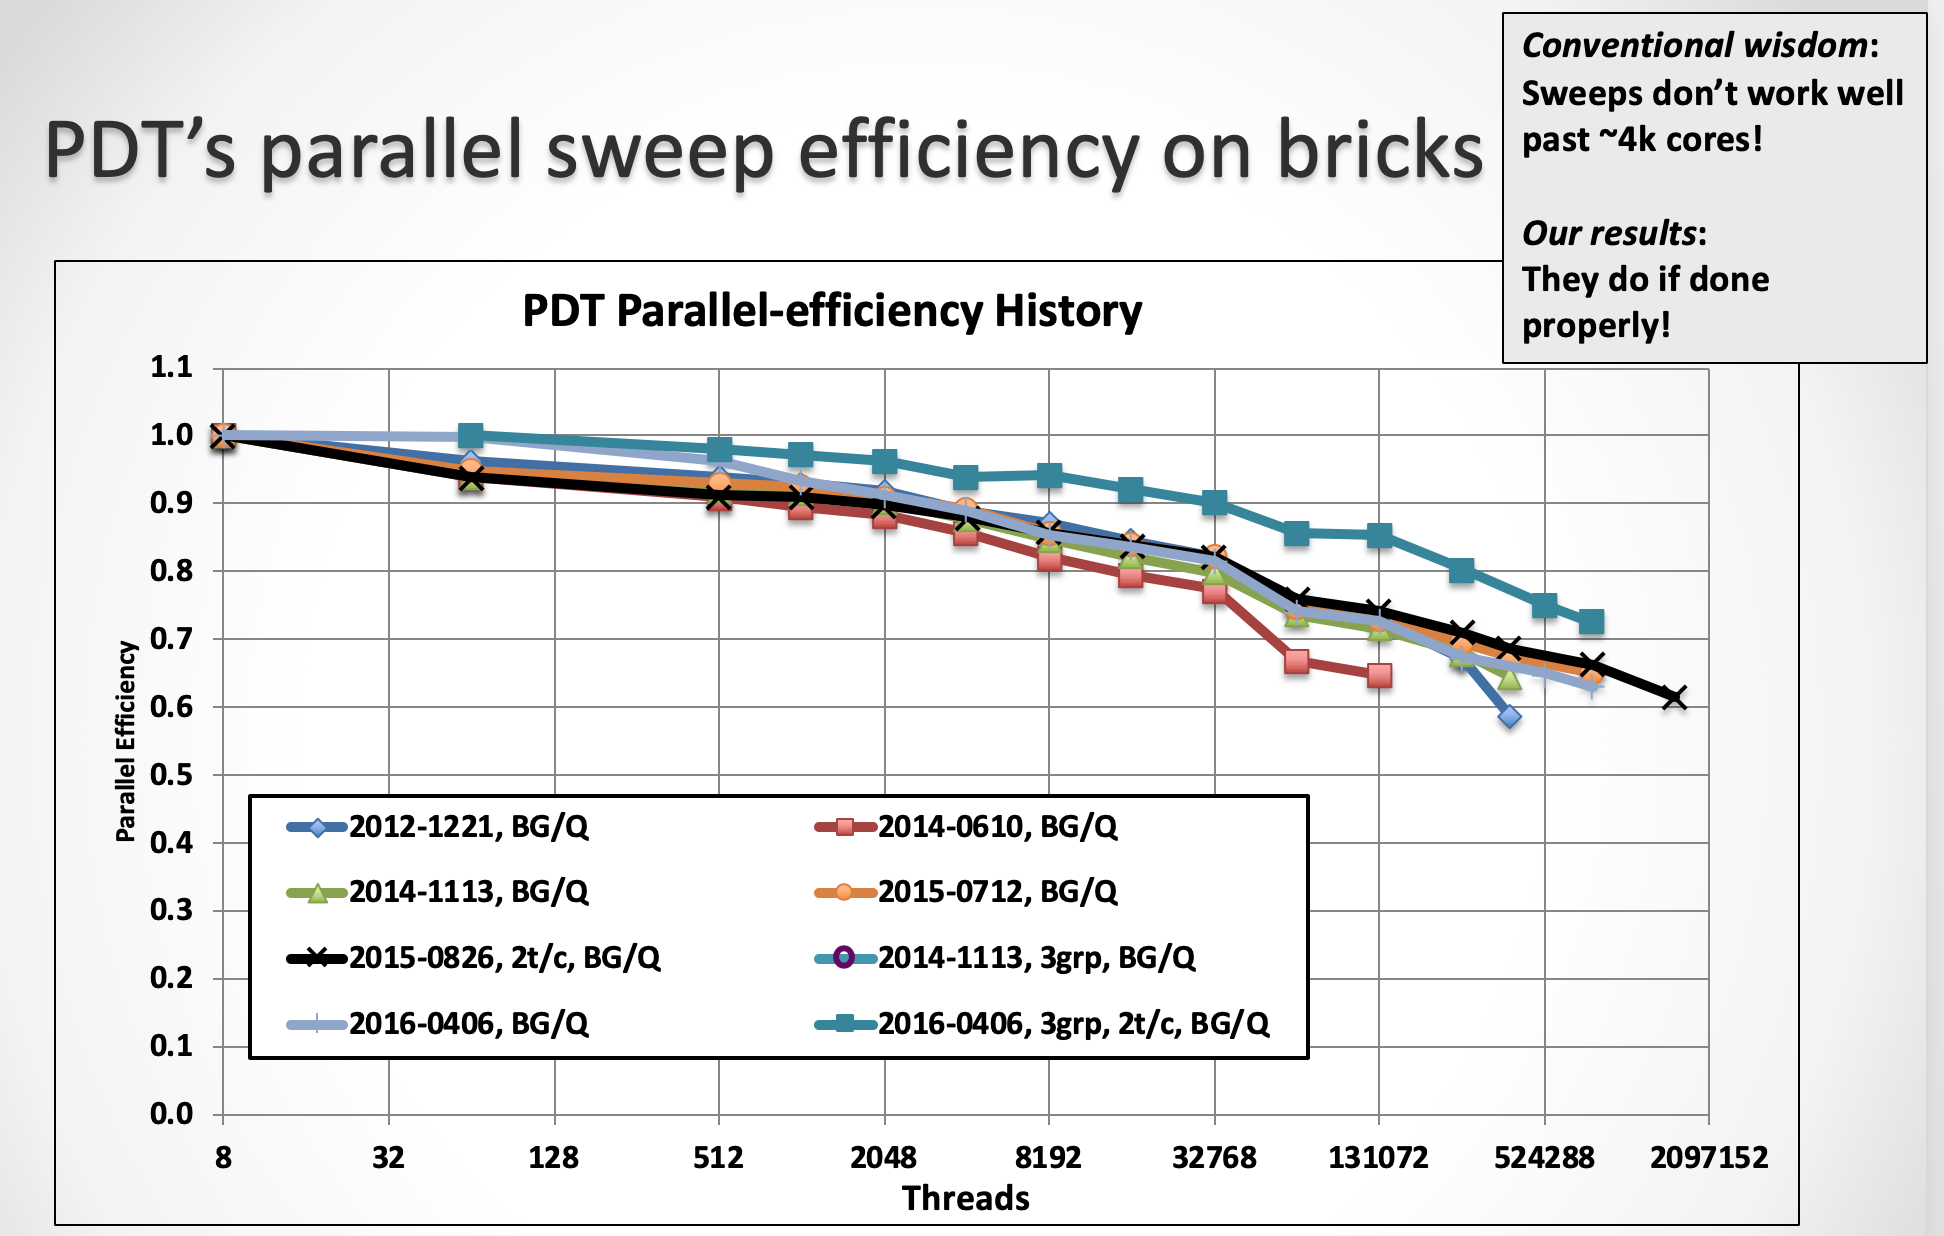
\includegraphics[scale=0.2]{../../figures/sweep_scale2b.png}
	\end{center}
	\item Structured meshes are limiting when modeling complex geometries.
	\item Unstructured meshes introduce unbalanced partitions. 
	\item PDT (Texas A\&M's massively parallel transport code) has two load balancing algorithms that repartition the mesh in order to obtain a roughly equivalent amount of cells per processor. 
\end{itemize}
\end{block}
\end{frame}
%%%%%%%%%%%%%%%%%%%%%%%%%%%%%%%%%%%%%%%%%%%%%%%%%%%%%%%%%%%%%%%%%%

\begin{frame}[t]\frametitle{Transport Sweeps}
\vspace{-2mm}
\begin{block}{}
\begin{itemize}
\item Transport equation is discretized over phase-space (space, direction, energy)
\item Discrete-ordinates in angle \textcolor{red}{+} Discontinuous FEM in space \textcolor{red}{+} upwind information at cell interfces \textcolor{red}{$\Longrightarrow$} solution one cell/one direction at a time,aka, \textbf{transport sweeps}
%\begin{equation}
%\vo_m \cdot \vec\nabla \psi_m^{(\ell+1)}(\vr) + \Sigma_t \psi_m^{(\ell+1)}(\vr) = q_m^{(\ell)}(\vr),
%\label{iteration}
%\end{equation}
%\begin{itemize}
%\item The domain is meshed, allowing one cell at a time to be solved.
%\item The solution across a cell interface is connected based on an upwind approach, allowing cells to be solved one at a time.
\end{itemize}
\end{block}

\begin{block}{\tcr{Structured-grid} sweeps}
\begin{figure}
	\centering
		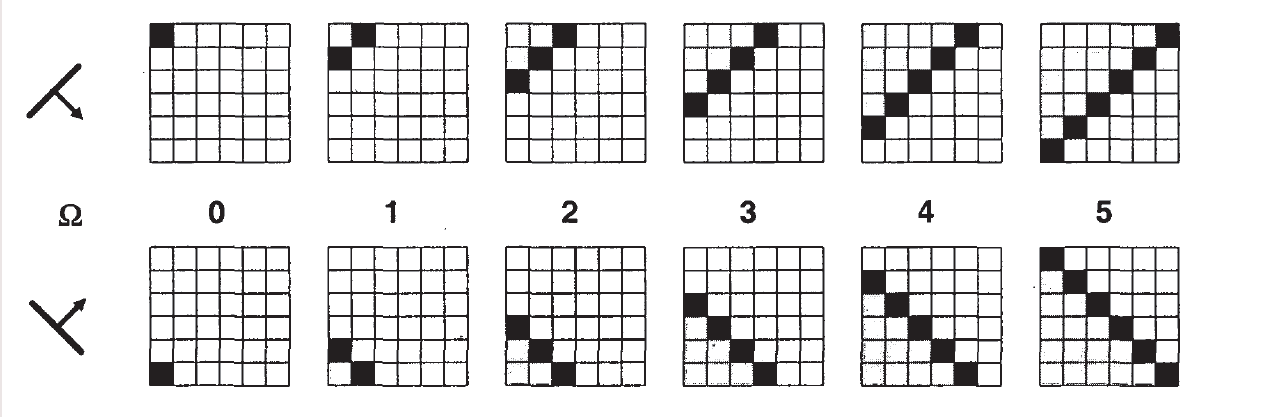
\includegraphics[scale=0.2]{../../figures/sweep_struct.png}
\end{figure}
\end{block}

\begin{block}{\tcr{Unstructured-grid} sweeps}
\begin{figure}
	\centering
		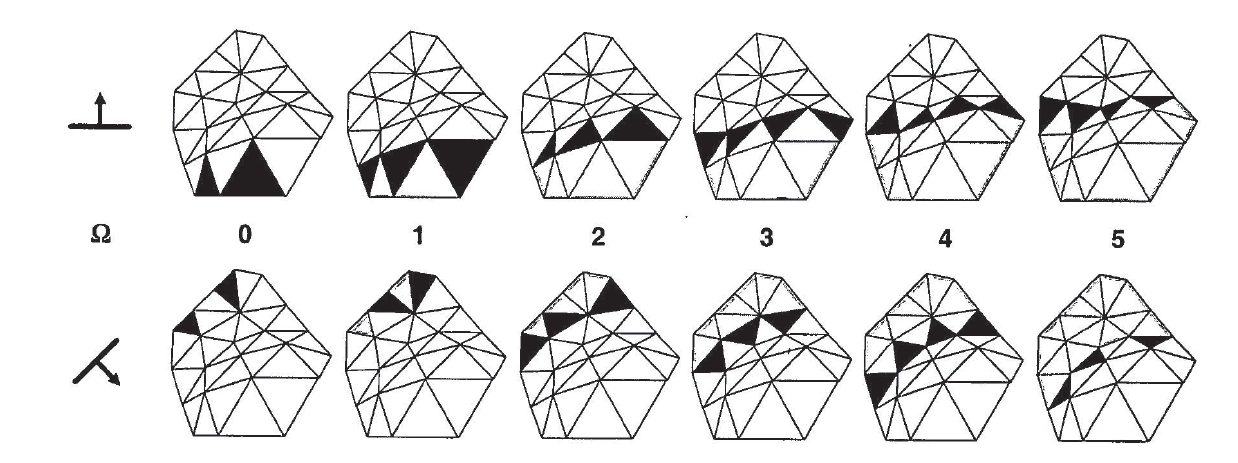
\includegraphics[scale=0.2]{../../figures/sweep_unstruct.png}
\end{figure}
\end{block}

\end{frame}
%%%%%%%%%%%%%%%%%%%%%%%%%%%%%%%%%%%%%%%%%%%%%%%%%%%%%%%%%%%%%%%%%%
%-------------------------------------------------------------------
\begin{frame}{Provably Optimal Parallel Transport Sweeps On Structured Grids (Adams \& Adams)}


\begin{block}{Ingredients for optimality}
\begin{enumerate}
\item spatial domain decomposition distributes the domain across processors (e.g., $P_x \times P_y \times P_z$),
\tcm{partition = dividing the domain among processors}
\item \tcm{aggregation} lumps fine-grained computations into ``tasks''
\begin{itemize}
\item cell-sets
\item angle-sets
\item energy-group-sets
\end{itemize}
\item \tcm{scheduling:} choosing which task of the graph to execute if more than one is available.
\end{enumerate}
\end{block}

\begin{center}
%\includegraphics[scale=0.3]{\FigDir/sweep_multi_angle}
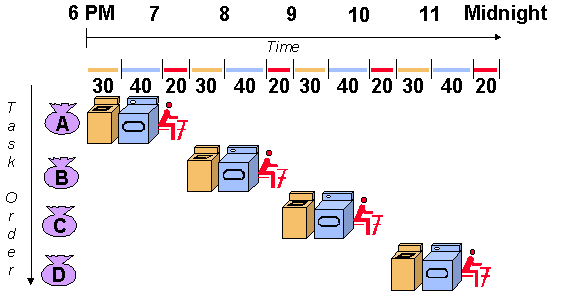
\includegraphics[scale=0.3]{../../figures/laundry1.png}
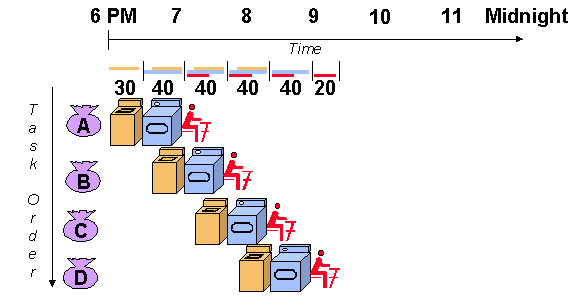
\includegraphics[scale=0.3]{../../figures/laundry2.png}
\end{center}
\end{frame}

%-------------------------------------------------------------------
\begin{frame}{Provably Optimal Parallel Transport Sweeps}
\vspace{-2mm}
\begin{block}{Usefulness of a performance model}
\begin{enumerate}
\item When a (deterministic) scheduling algorithm is well understood, stage counts can be \fbox{predicted} with significant benefits.
\item In a nutshell, we have a \tcr{performance model} that depends on the processor partition, the aggregation factors, the scheduler, and \tcr{machine parameters} (grind time, latency). \\
PDT runs in {\bf \tcr{auto-mode}} and picks the optimal solution to traverse the TDG's.
% \[
% T_{\text{sweeps}} = N_\text{stages}
% \left( T_\text{work function} + 3T_\text{latency} +
% N_\text{bytes}T_\text{band-width} + A_x A_y A_z N_\text{?}
% \left( T_\text{cell} + A_m
% \left(T_\text{mom}+A_g T\text{g}
% \right)\right)\right)
% \]
\end{enumerate}
\end{block}

%\begin{block}{Optimality}
%\ben
%\item Execute the sweeps in the \tcr{fewest possible stages}
%\item Have a performance model (function of problem dimension, machine parameters, partition, aggregation)
%\item Have an optimization of the performance model to select the best aggregation factors
%\een
%\end{block}

%\end{frame}
%%%%%%%%%%%%%%%%%%%%%%%%%%%%%%%%%%%%%%%%%%%%%%%%%%%%%%%%%%%%%%%%%%%%%
%%-------------------------------------------------------------------
%\begin{frame}{Parallel Transport Sweeps}

\vspace{-2mm}
\begin{block}{Number of Tasks}
\be
% N_{tasks} = \frac{ N_x N_y N_z 8M G}{A_x A_y A_z A_m A_g P_x P_y P_z}
N_{tasks} = \frac{ N_x N_y N_z}{A_x A_y A_z } \times \frac{8D}{A_d}
\times \frac{G}{A_g} \times \frac{1}{P_x P_y P_z}
\ee
\end{block}

\vspace{-2mm}
\begin{block}{Number of Parallel stages}
\be
%N_{stages} = N_{tasks} + \tcr{N_{idle}} =  N_{tasks} + \tcr{P_x+P_y+P_z-6}
N_{stages} = N_{tasks} + \tcr{N_{idle}} =  N_{tasks} +
\tcr{2\left( \frac{P_x}{2}-1+\frac{P_y}{2}-1+\frac{P_z}{2}-1 \right)}
\ee
The ``depth-of-graph'' scheduling algorithm prioritizes tasks based on the number of downstream dependencies and yields the smallest $N_{stages}$.
\end{block}
%
An optimal scheduling algorithm executes the sweeps in the fewest possible stages (limit the idle time of pieces of work far form boundaries)
%\be
%\epsilon = \frac{N_{tasks}T_{task}}{N_{stages}(T_{task}+T_{comm})} =
%\frac{1}{\left( 1+\frac{N_{idle}}{N_{tasks}}\right) \left( 1+\frac{T_{comm}}{T_{task}}\right)}
%\ee

\end{frame}
%%%%%%%%%%%%%%%%%%%%%%%%%%%%%%%%%%%%%%%%%%%%%%%%%%%%%%%%%%%%%%%%%%%%


%
%\begin{frame}[t]\frametitle{Parallel Transport Sweeps}
%
%\begin{block}{A parallel sweep algorithm is defined by three properties:}
%\begin{itemize}
%\item partitioning: dividing the domain among available processors,
%\item aggregation: grouping cells, directions, and energy groups into tasks,
%\item scheduling: choosing which task to execute if more than one is available.
%\end{itemize}
%\end{block}
%\end{frame}
%%%%%%%%%%%%%%%%%%%%%%%%%%%%%%%%%%%%%%%%%%%%%%%%%%%%%%%%%%%%%%%%%%

%\begin{frame}[t]\frametitle{Tie Breaking in PDT}
%
%\begin{block}{If two or more tasks reach a processor at the same time, PDT employs a tie breaking strategy:}
%
%\begin{enumerate}
%	\item The task with the greater depth-of-graph remaining (simply, more work remaining) goes first.
%	\item If the depth-of-graph remaining is tied, the task with $\Omega_x > 0$ wins.
%	\item If multiple tasks have $\Omega_x > 0$, then the task with $\Omega_y > 0$ wins.
%	\item If multiple tasks have $\Omega_y > 0$, then the task with $\Omega_z > 0$ wins.
%\end{enumerate}
%\end{block}
%\end{frame}
%%%%%%%%%%%%%%%%%%%%%%%%%%%%%%%%%%%%%%%%%%%%%%%%%%%%%%%%%%%%%%%%%%

\begin{frame}[t]\frametitle{Unstructured Meshing in PDT}
  \begin{block}{}
    \begin{itemize}
      \item PDT using unstructured meshes has been a priority since early 2014. 
      \item Unstructured meshes allow for simulation of a wider and more general variety of problems.
      \item Three unstructured mesh types are supported in PDT:
        \begin{itemize}
          \item Triangle (2D and 2D extruded triangular/prismatic meshes).
          \item Spiderweb (2D and 2D extruded prismatic meshes).
          \item Cubit/OpenFOAM (fully unstructured 3D meshes).
        \end{itemize}
    \end{itemize}
  \end{block}
  \centering
  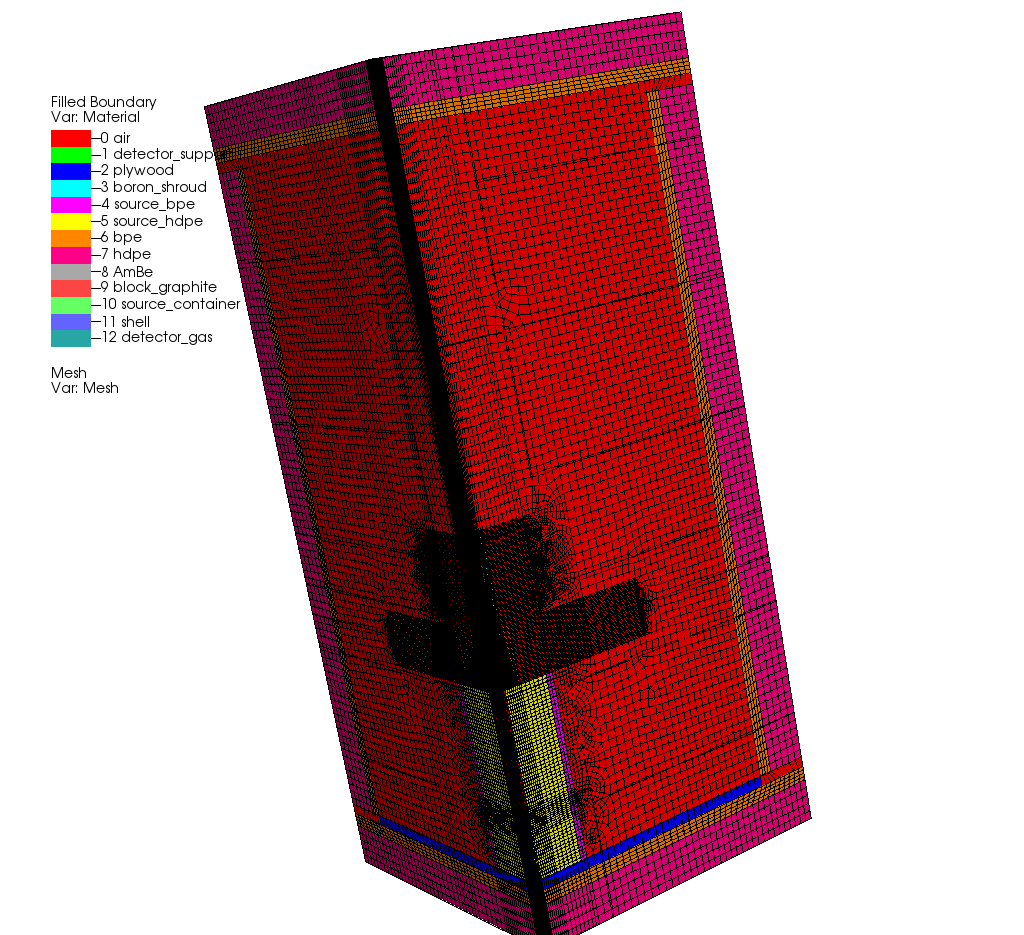
\includegraphics[scale=0.14]{../../figures/im1_228.png}
\end{frame}
%%%%%%%%%%%%%%%%%%%%%%%%%%%%%%%%%%%%%%%%%%%%%%%%%%%%%%%%%%%%%%%%%%

\begin{frame}[t]\frametitle{Partitioning in PDT}
\begin{block}{Partitioning for Unstructured Meshes}
\begin{itemize}
\item ``Cut lines'' in 2D (cut planes for 3D) are used to slice through the mesh in the $x$, $y$, and $z$ dimensions.
\item The cut planes form brick partitions, called subsets, that have unstructured meshes inside of them. 
\item The subsets are distributed amongst the processors.
\end{itemize}
\end{block}
  \begin{block}{PWLD}
     Using Piece-Wise Linear Discontinuous finite element basis functions, we can solve the transport equation for arbitrary and degenerate polyhedra.
  \end{block}
  \centering
  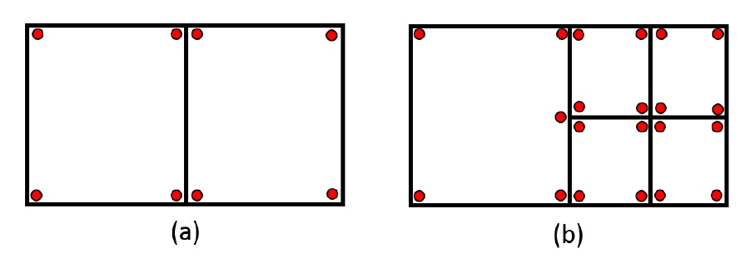
\includegraphics[scale=0.5]{../../figures/degen_penta.png}
  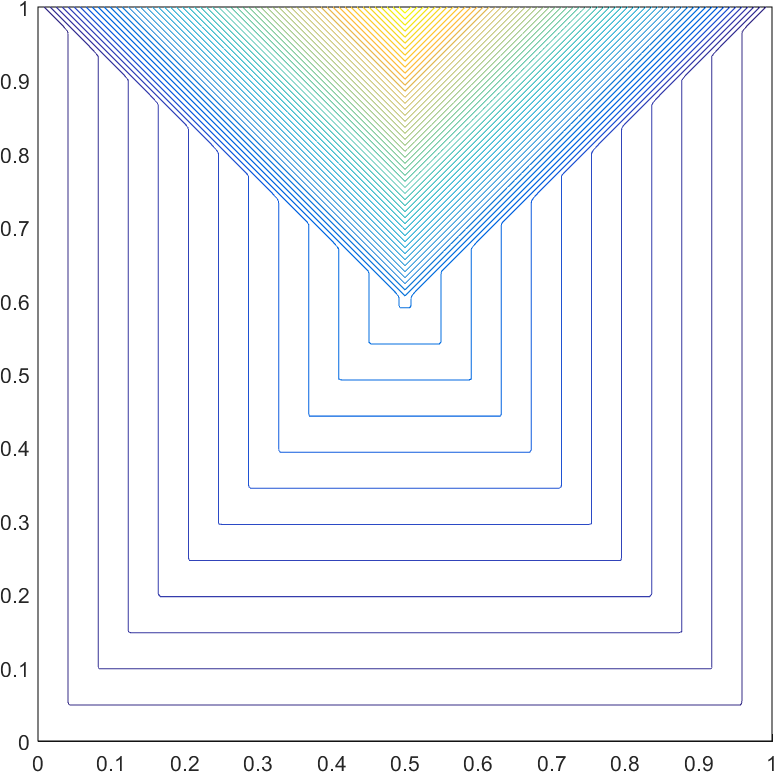
\includegraphics[scale=0.25,angle=270,origin=c]{../../figures/deg_square_PWLD1_contour_b4.png}
\end{frame}
%%%%%%%%%%%%%%%%%%%%%%%%%%%%%%%%%%%%%%%%%%%%%%%%%%%%%%%%%%%%%%%%%%

\begin{frame}[t]\frametitle{Partitioning in PDT}
  
  \begin{columns}
    \column{0.5\textwidth}
    \begin{minipage}[c][0.4\textheight][c]{\linewidth}
      \centering
      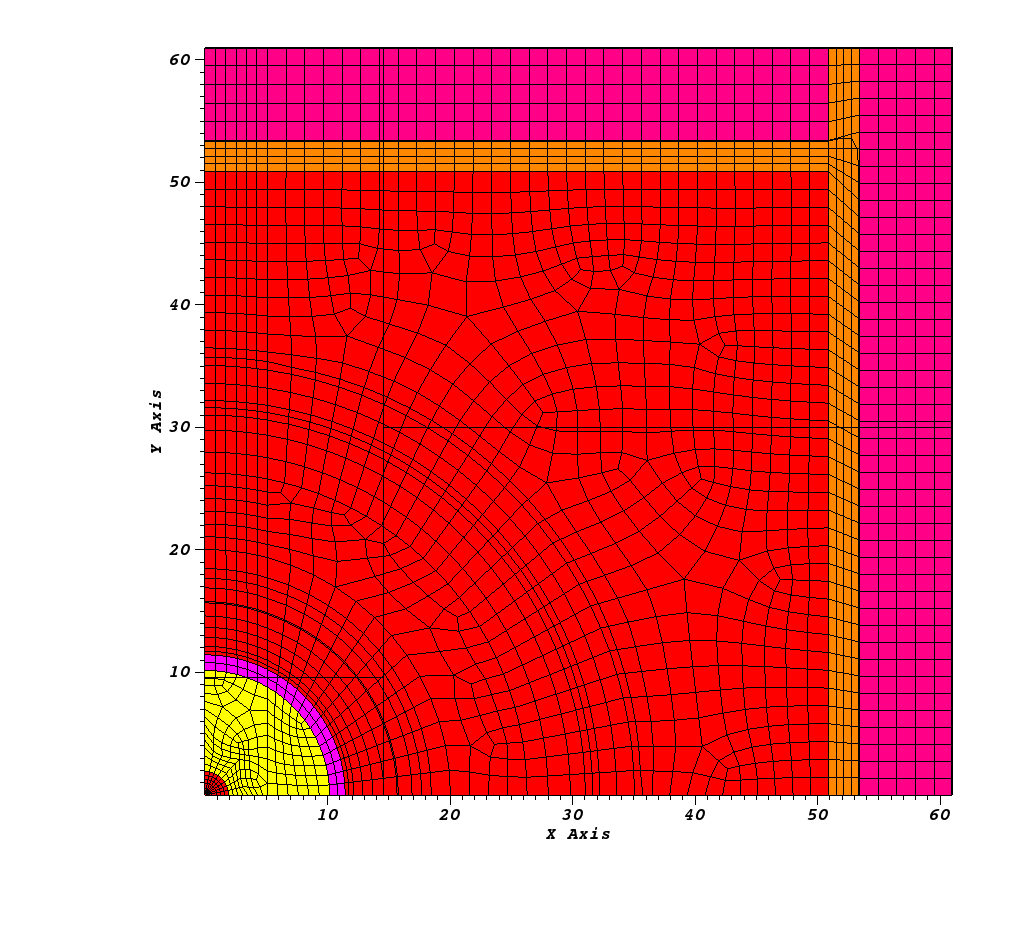
\includegraphics[scale=0.14,trim={0.95in 0.64in 0.35in 0.44in},clip]{../../figures/im1_cubit_slice.png}
    \end{minipage}
    
    \begin{minipage}[c][0.4\textheight][c]{\linewidth}
      \centering
      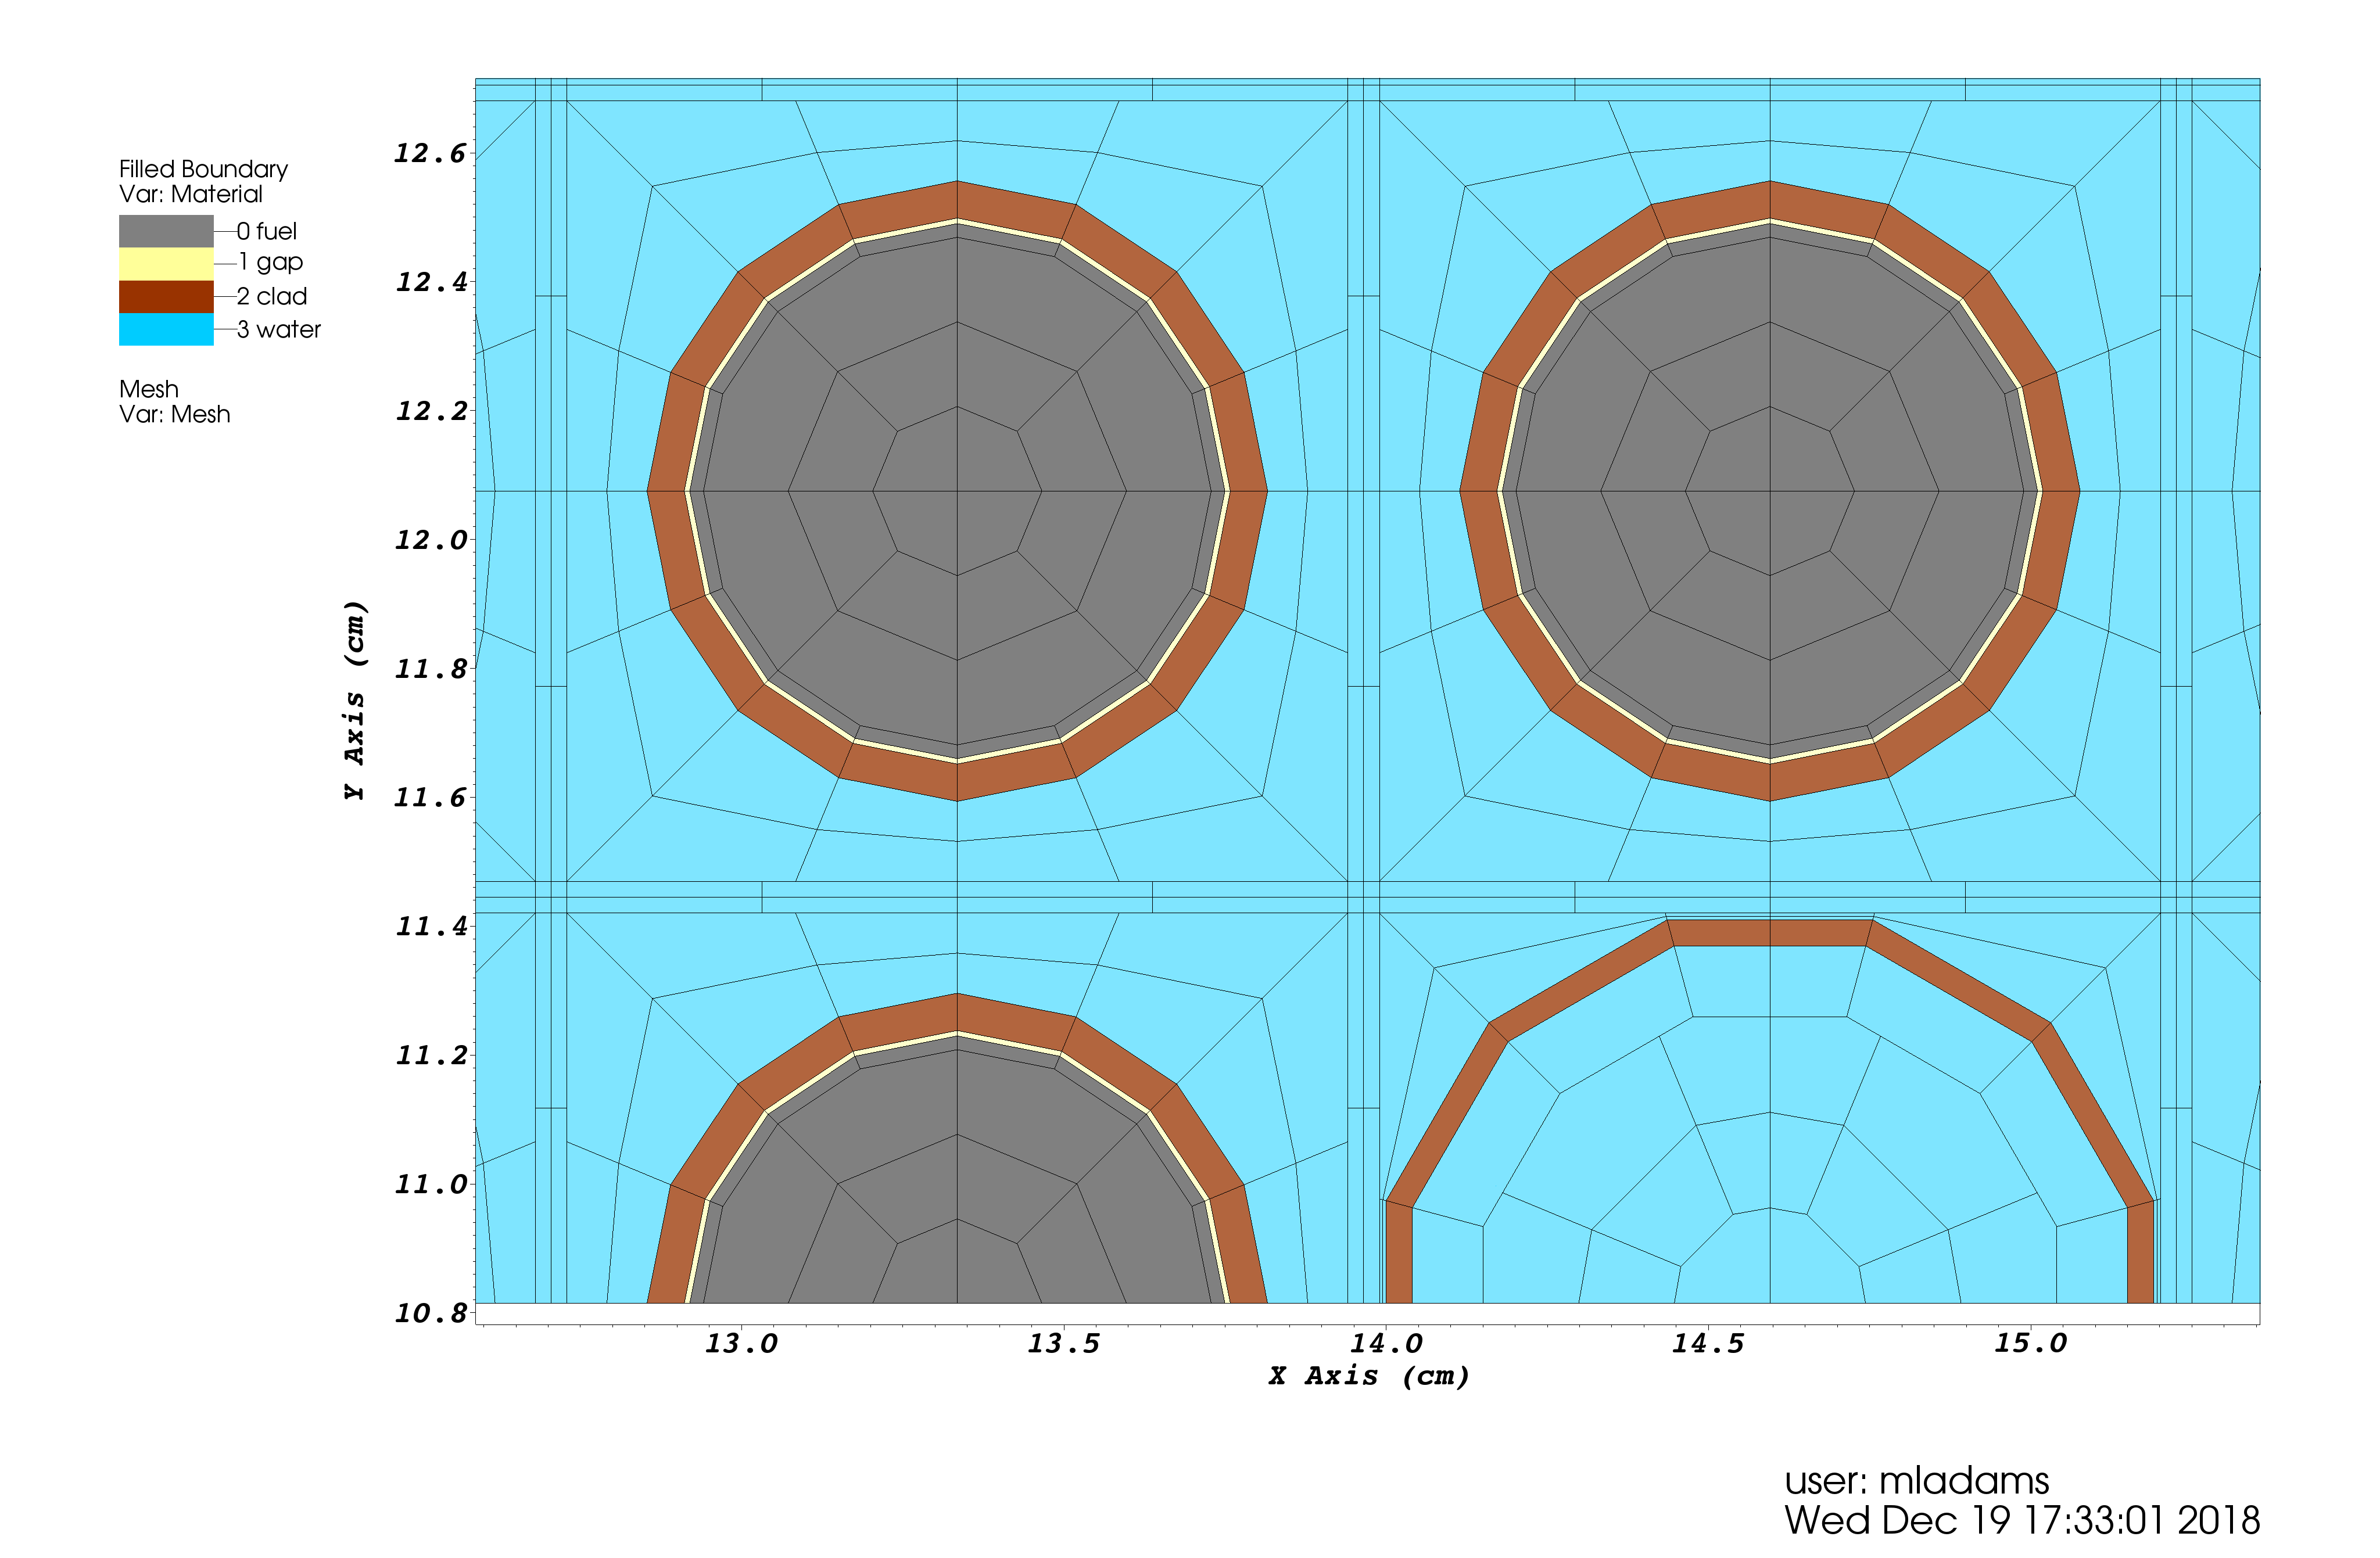
\includegraphics[scale=0.05]{../../figures/FuelAndGuideZoom.png}
    \end{minipage}
    
    \column{0.5\textwidth}
      \vspace{-3mm}
%    \begin{minipage}[c][0.4\textheight][c]{\linewidth}
    \begin{minipage}[c][0.4\textheight][c]{\linewidth}
      \centering
      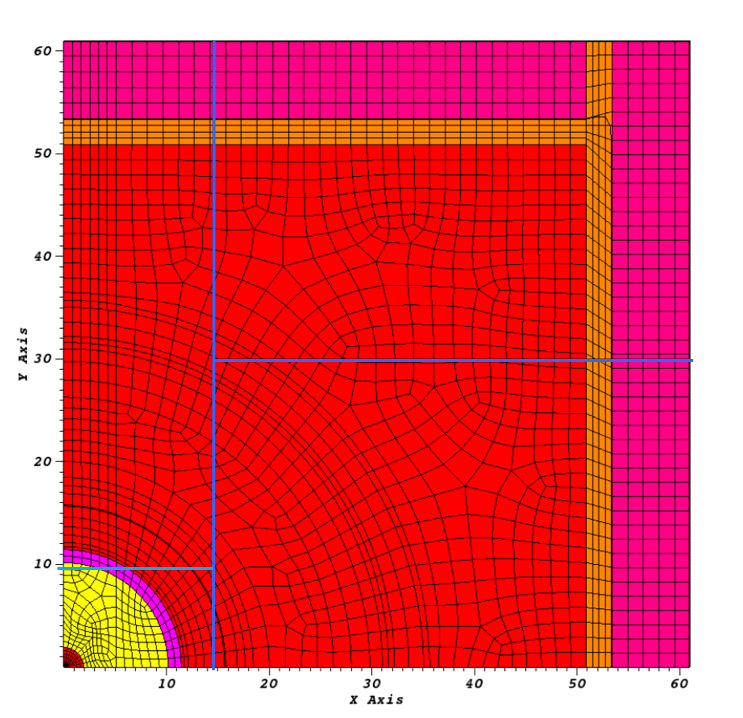
\includegraphics[scale=0.4,trim={0.95in 0.64in 0.35in 0.44in},clip]{../../figures/im1_cubit_slice_v2.png}
    \end{minipage}
%      \begin{block}{}
%        PWLD allows us to solve these partitioned arbitrary and degenerate meshes.
%      \end{block}
%    \end{minipage}
    \begin{minipage}[c][0.4\textheight][c]{\linewidth}
      \centering
      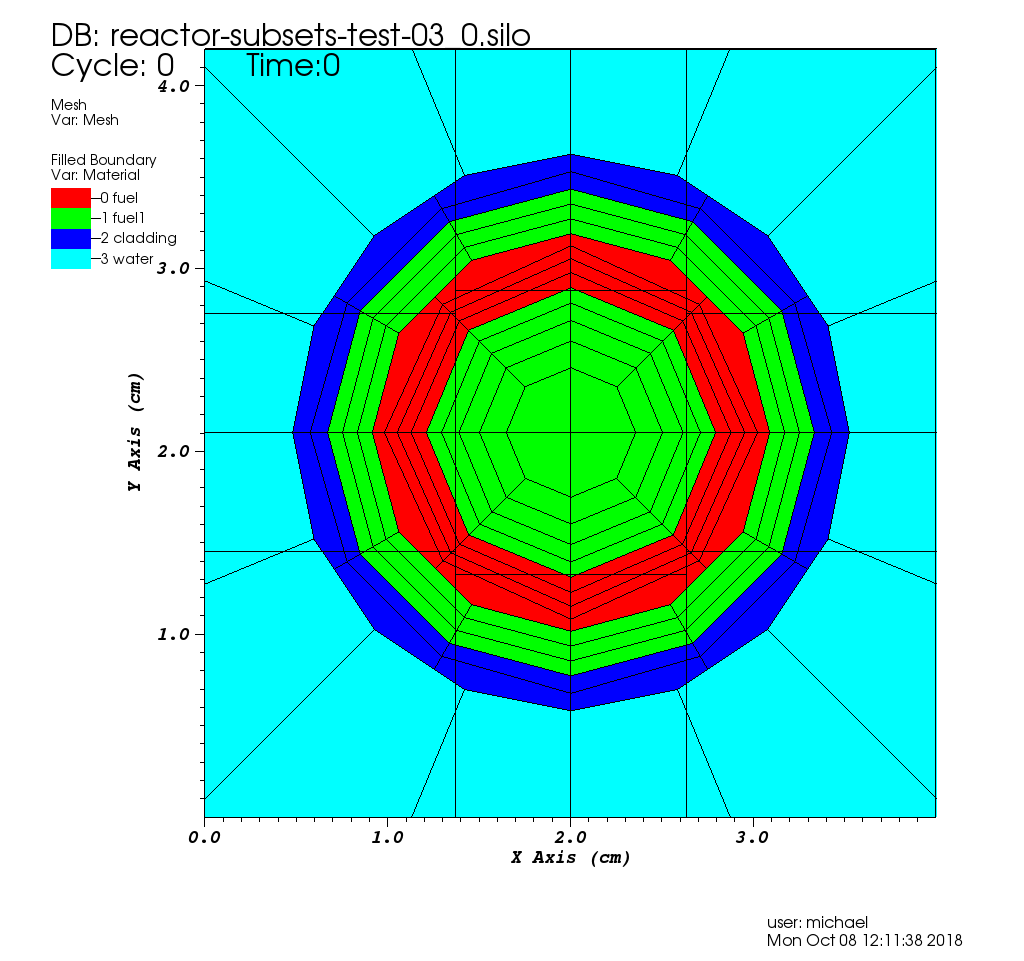
\includegraphics[scale=0.125]{../../figures/spiderweb4.png}
    \end{minipage}
  \end{columns}
\end{frame}
%%%%%%%%%%%%%%%%%%%%%%%%%%%%%%%%%%%%%%%%%%%%%%%%%%%%%%%%%%%%%%%%%%

\section{Load Balancing}
\subsection{}

\begin{frame}[t]\frametitle{Load Balancing}
\begin{block}{}
  \begin{itemize}
    \item The load balancing by dimension algorithm expands upon load balancing work presented at M\&C 2017.
    \item The algorithm looks to achieve an equivalent number of cells across all subsets by \tcr{placing cut lines/planes  when creating subsets}.
    \item Placement of cut lines/planes done by analyzing the CDF of mesh density function integrated over the spatial other dimensions (example below).
  \end{itemize}		
\end{block}
\begin{minipage}[c]{0.49\textwidth}
\centering
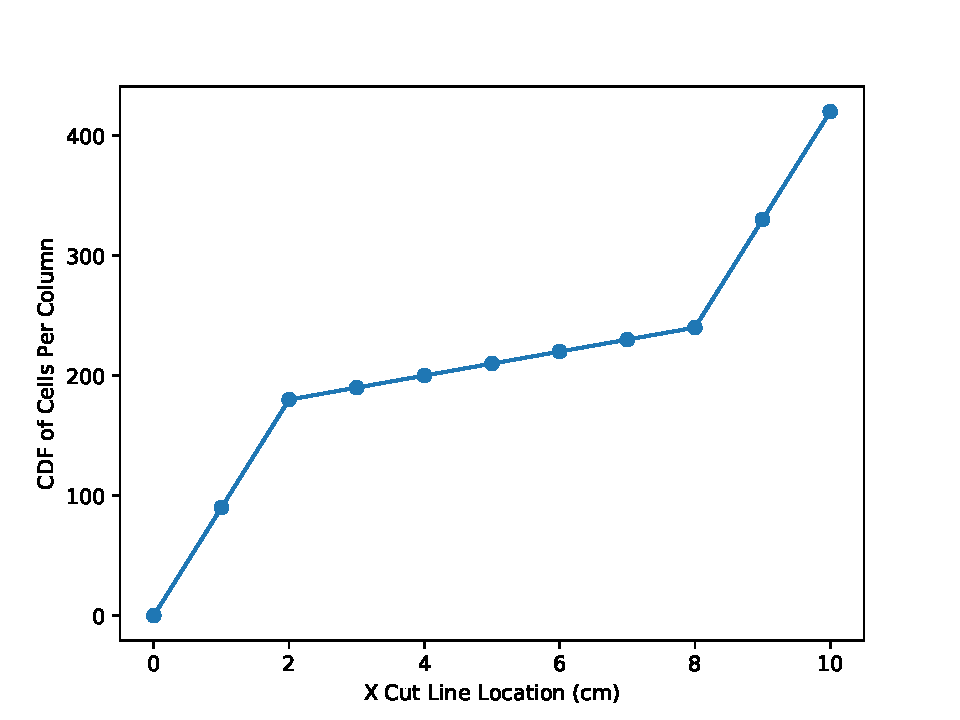
\includegraphics[scale=0.3]{../../figures/spiderweb_redistribute_before_sparse.pdf}
\end{minipage}
\begin{minipage}[c]{0.49\textwidth}
\centering
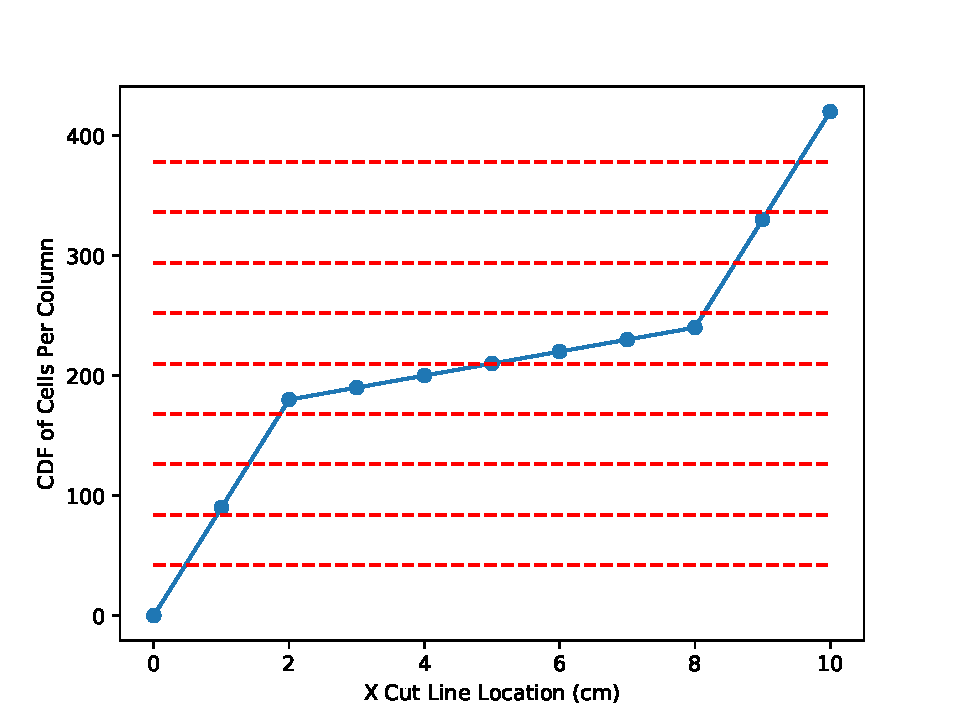
\includegraphics[scale=0.3]{../../figures/spiderweb_redistribute_after_sparse.pdf}
\end{minipage}
\end{frame}
%%%%%%%%%%%%%%%%%%%%%%%%%%%%%%%%%%%%%%%%%%%%%%%%%%%%%%%%%%%%%%%%%%

\begin{frame}[t]\frametitle{Load Balancing}
\begin{minipage}[c]{0.49\textwidth}
\centering
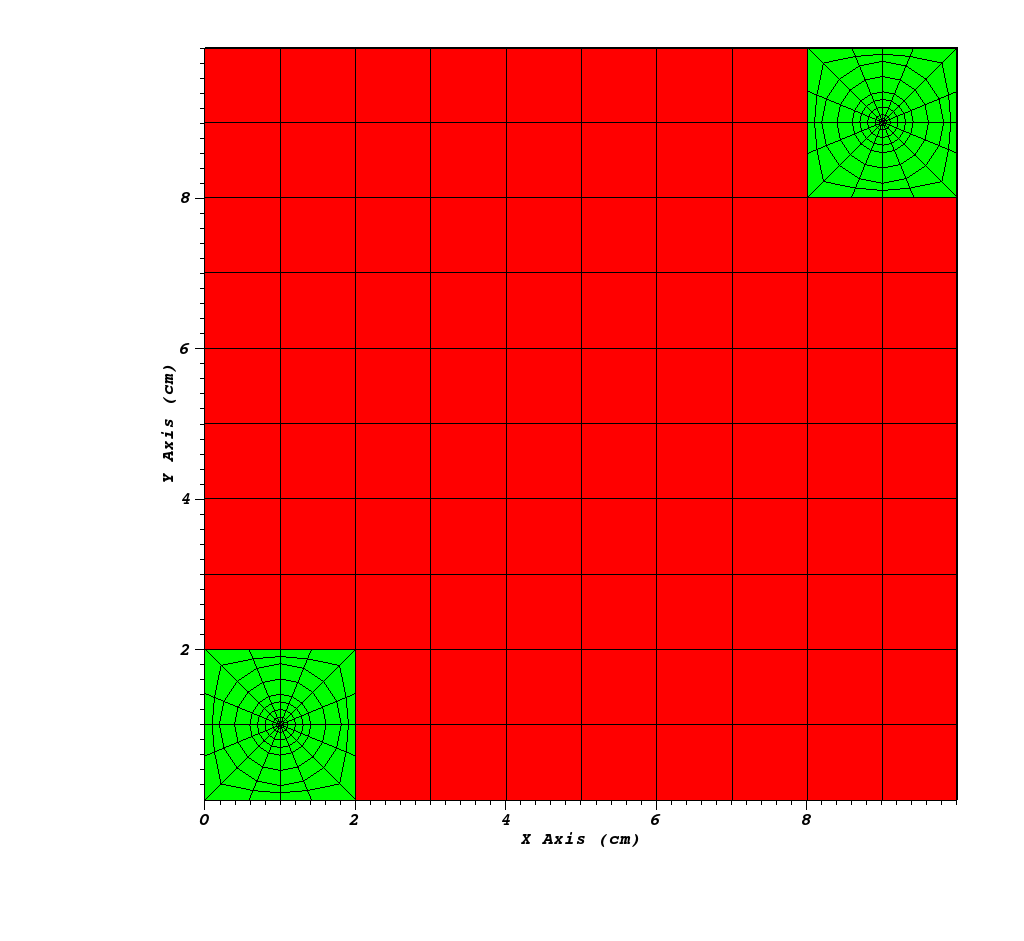
\includegraphics[scale=0.2,trim={0.95in 0.64in 0.35in 0.44in},clip]{../../figures/spiderweb_sparse.png}\\
\centering
$f = 9.7619$
\end{minipage}
\begin{minipage}[c]{0.49\textwidth}
\centering
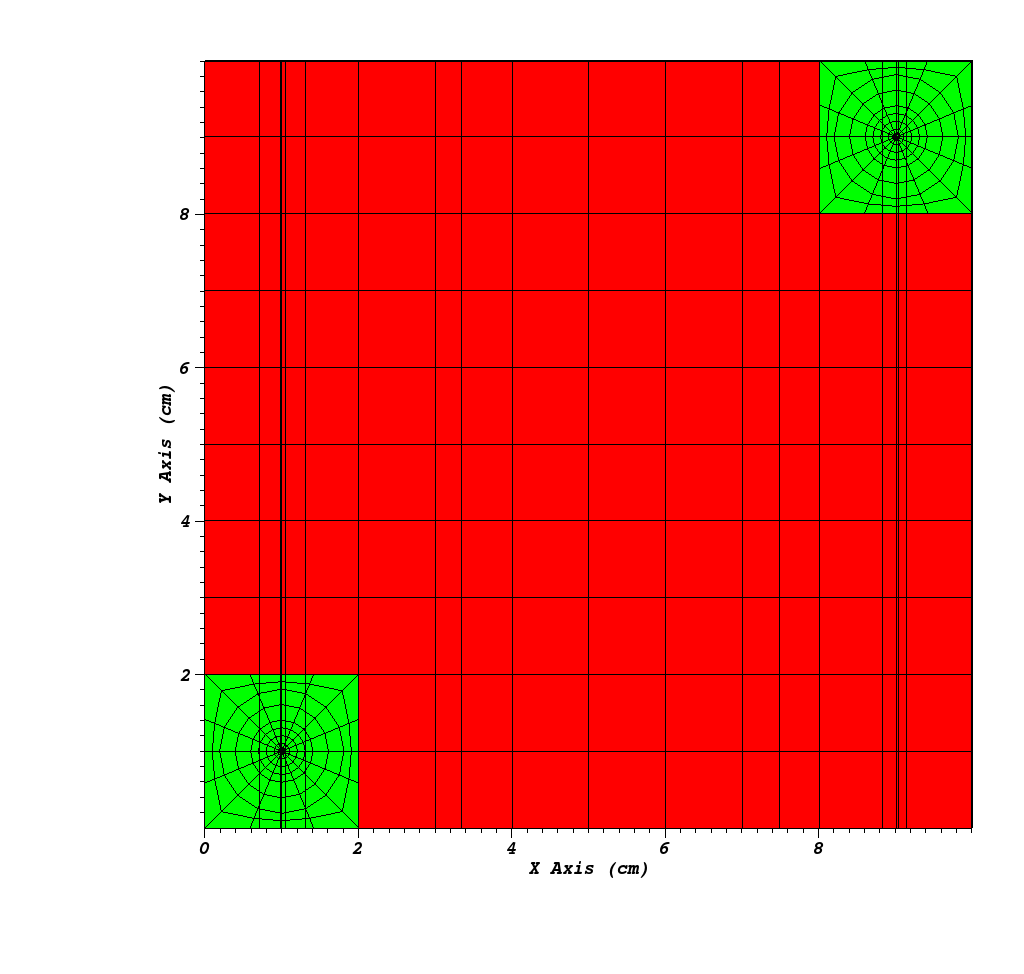
\includegraphics[scale=0.2,trim={0.95in 0.64in 0.35in 0.44in},clip]{../../figures/sparse_spiderweb_lb.png}\\
\centering
$f = 6.85358$
\end{minipage}
\end{frame}
%%%%%%%%%%%%%%%%%%%%%%%%%%%%%%%%%%%%%%%%%%%%%%%%%%%%%%%%%%%%%%%%%%%%

\begin{frame}[t]\frametitle{Load Balancing By Dimension (LBD)}
\begin{block}{}
LBD: a more efficient load-balancing approach:\\
Take a 3D mesh.
\begin{enumerate}
    \item  Slice it in axial layers such that each layer has about the same \# of cells.
    \item  Then, for each layer, slice it in columns such that each column has about the same \# of cells.
    \item Then, for each column, slice it in blocks such that each block has about the same \# of cells. 
\end{enumerate}
In practice, we often achieve close to perfect load balance. (typical imbalance is < 1\%)
 %on that new slide, I would split the bottom half on 2 columns: left column some text from slide 15, on the right, the figure from slide 15
\end{block}
\begin{minipage}[c]{0.49\textwidth}
\centering
 \begin{block}{Theoretical motivation for LBD}
  \begin{itemize}
    \item Consider simple 2D layout with $M$ unaligned subsets of high mesh density that each have $N$ cells.
    \item There are $M^2$ subsets, but only M have much work.
    \item Load Imbalance Factor $= \frac{N}{(MN+C)/M^2} \xrightarrow{N\to \infty} \frac{N}{N/M} = M$
  \end{itemize}
  \end{block}
\end{minipage}
\begin{minipage}[c]{0.49\textwidth}
\centering
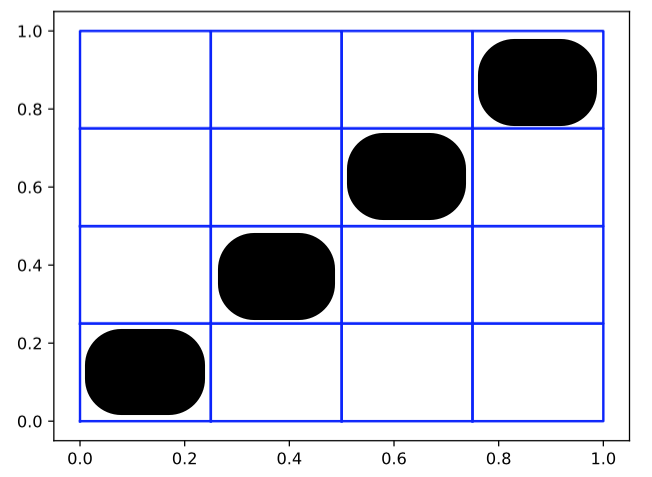
\includegraphics[scale=0.2]{../../figures/theoretical_plot.png}
\end{minipage}
\end{frame}
%%%%%%%%%%%%%%%%%%%%%%%%%%%%%%%%%%%%%%%%%%%%%%%%%%%%%%%%%%%%%%%%%%

\begin{frame}[t]\frametitle{Load Balancing By Dimension}

\vspace{2cm}
\begin{minipage}[c]{0.32\textwidth}
\centering
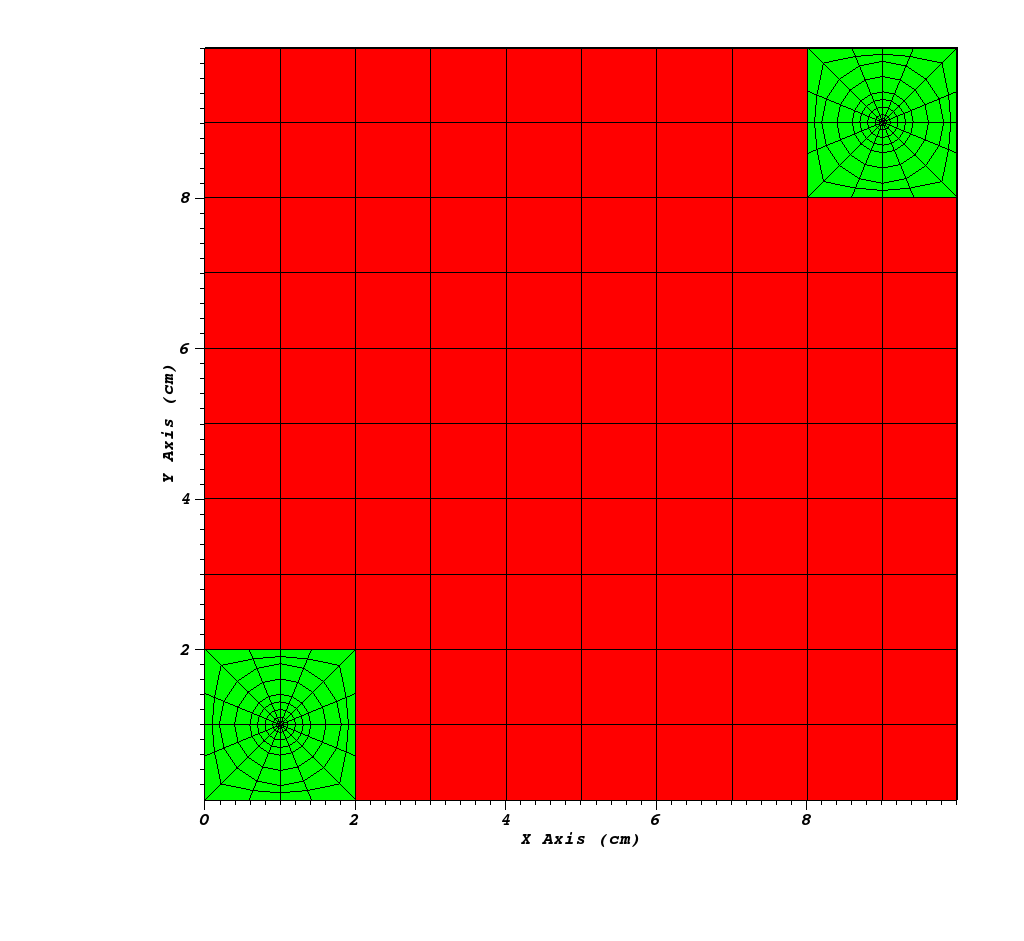
\includegraphics[scale=0.12,trim={0.95in 0.64in 0.35in 0.44in},clip]{../../figures/spiderweb_sparse.png} \\
\centering
$f = 9.7619$
\end{minipage}
\begin{minipage}[c]{0.32\textwidth}
\centering
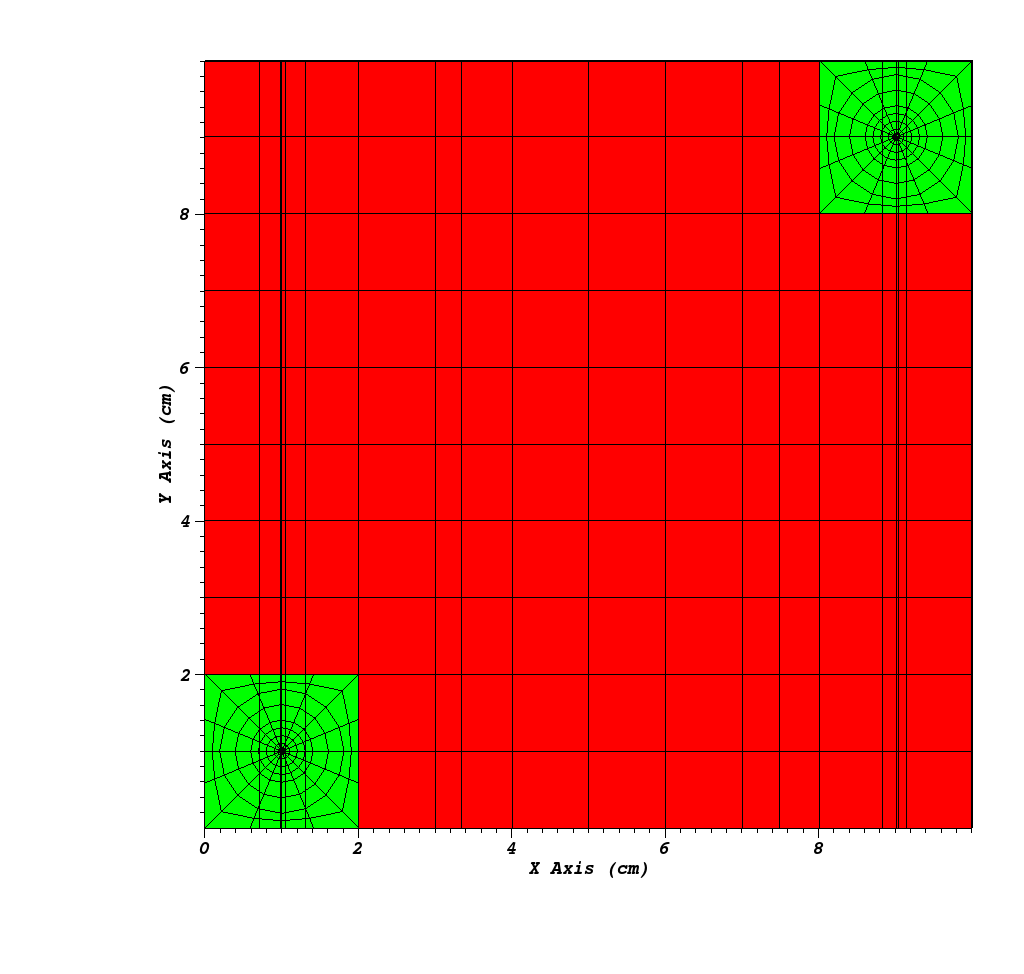
\includegraphics[scale=0.12,trim={0.95in 0.64in 0.35in 0.44in},clip]{../../figures/sparse_spiderweb_lb.png}\\
\centering
$f = 6.85358$
\end{minipage}
\begin{minipage}[c]{0.32\textwidth}
\centering
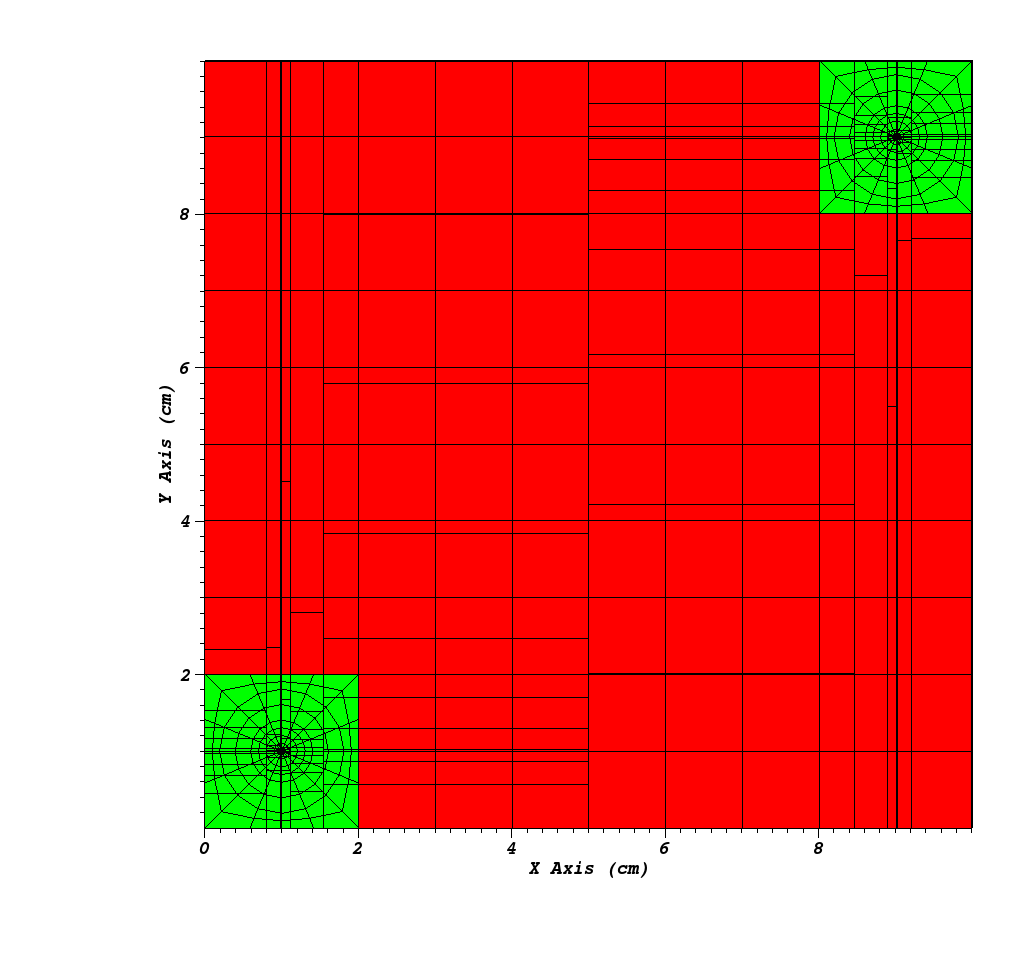
\includegraphics[scale=0.12,trim={0.95in 0.64in 0.35in 0.44in},clip]{../../figures/sparse_spiderweb_lbd.png} \\
\centering
$f = 1.49813$
\end{minipage}
\end{frame}
%%%%%%%%%%%%%%%%%%%%%%%%%%%%%%%%%%%%%%%%%%%%%%%%%%%%%%%%%%%%%%%%%%%%

\begin{frame}[t]\frametitle{Testing Load Balancing}
\begin{block}{}
\begin{itemize}
  \item This mesh was run through the load balancing and load balancing by dimension algorithm.
  \item The number of subsets ranged from 2 to 7 in both dimensions.
\end{itemize}
\end{block}
  \centering
  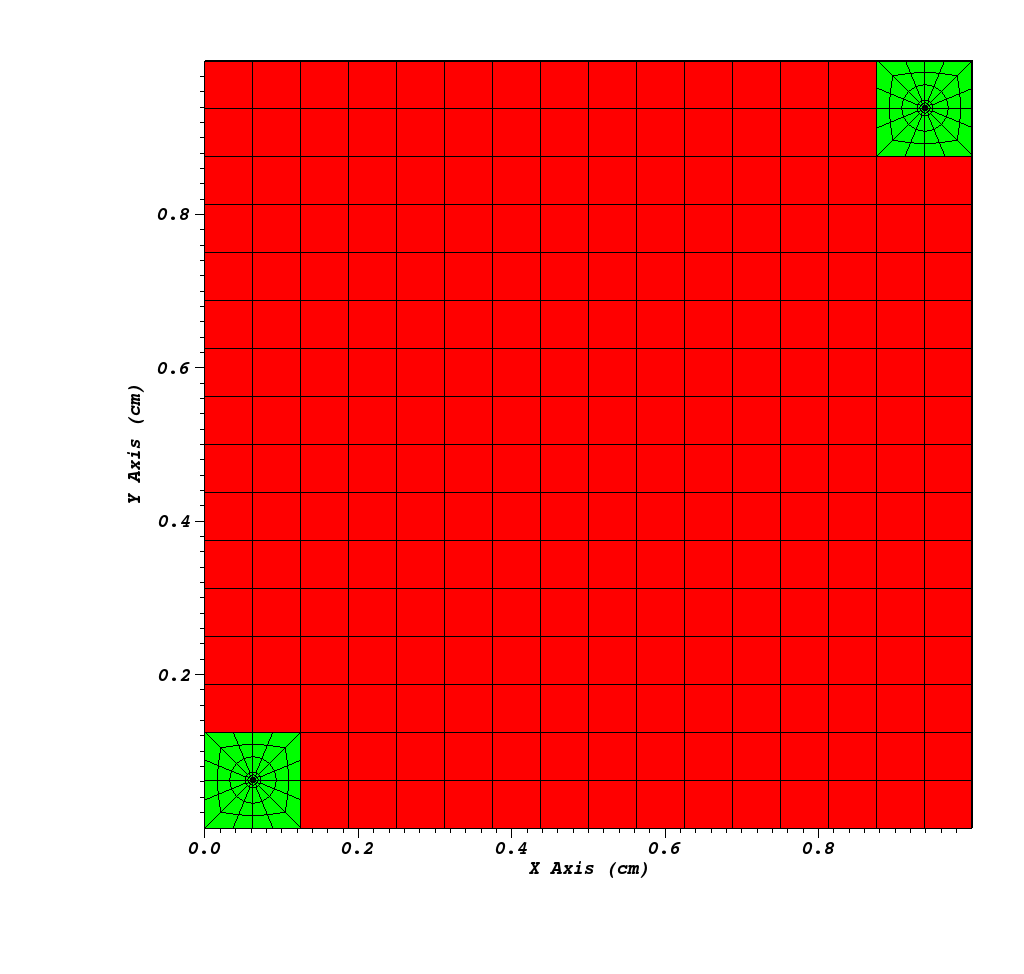
\includegraphics[scale=0.17,trim={2cm 0cm 1cm 1.3cm},clip]{../../figures/unbalanced_pins_refined.png}
\end{frame}
%%%%%%%%%%%%%%%%%%%%%%%%%%%%%%%%%%%%%%%%%%%%%%%%%%%%%%%%%%%%%%%%%%

\begin{frame}[t]\frametitle{Results of Load Balancing By Dimension}
\begin{minipage}[c]{0.6\textwidth}
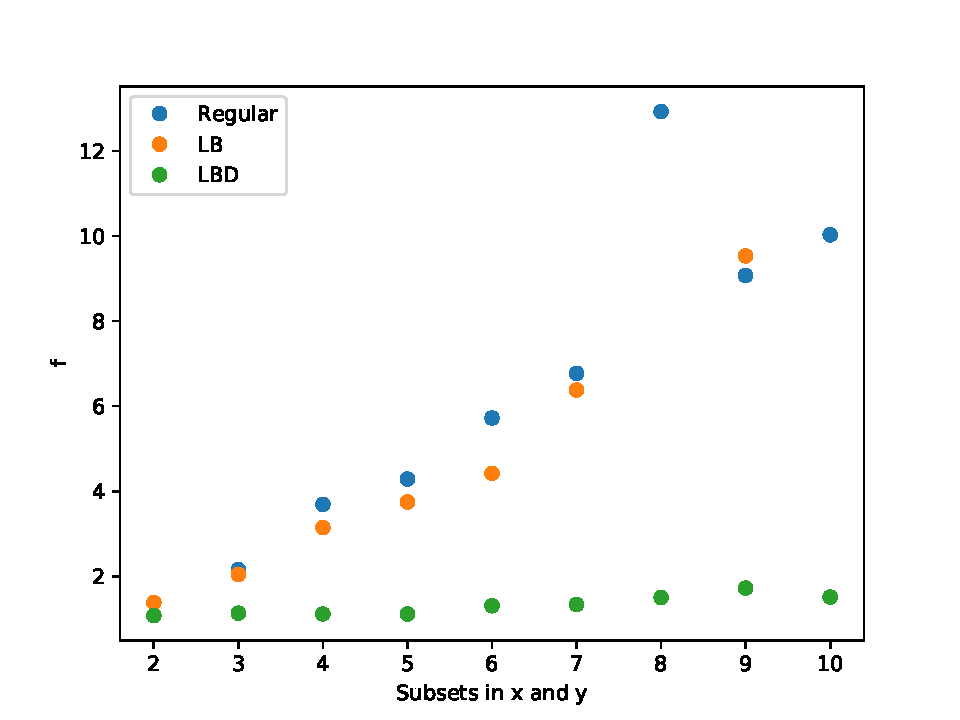
\includegraphics[scale=0.5]{../../figures/lbd_results.pdf} \\
\small Minimum LBD metric: 1.07692\\ Max LBD metric: 1.33636
\end{minipage}
\begin{minipage}[c]{0.38\textwidth}
  \centering
  \begin{table}[H]  
  \scalebox{0.9}{
    \begin{tabular}{c | c | c | c}
      \textbf{N} & \textbf{f\textsubscript{reg}} & \textbf{f\textsubscript{lb}} & \textbf{f\textsubscript{lbd}}  \\
      2&1.38462&1.384615&1.07692 \\ 
      3&2.15702&2.04545&1.13445 \\ 
      4&3.69231&3.1453&1.11498 \\ 
      5&4.28571&3.74564&1.11386 \\ 
      6&5.72143&4.42105&1.30796 \\ 
      7&6.77174&6.37778&1.33636 \\ 
    \end{tabular}}
  \end{table}
\end{minipage}
\end{frame}
%%%%%%%%%%%%%%%%%%%%%%%%%%%%%%%%%%%%%%%%%%%%%%%%%%%%%%%%%%%%%%%%%%

\begin{frame}[t]\frametitle{3D LBD, $f = 1.0199$}
\centering
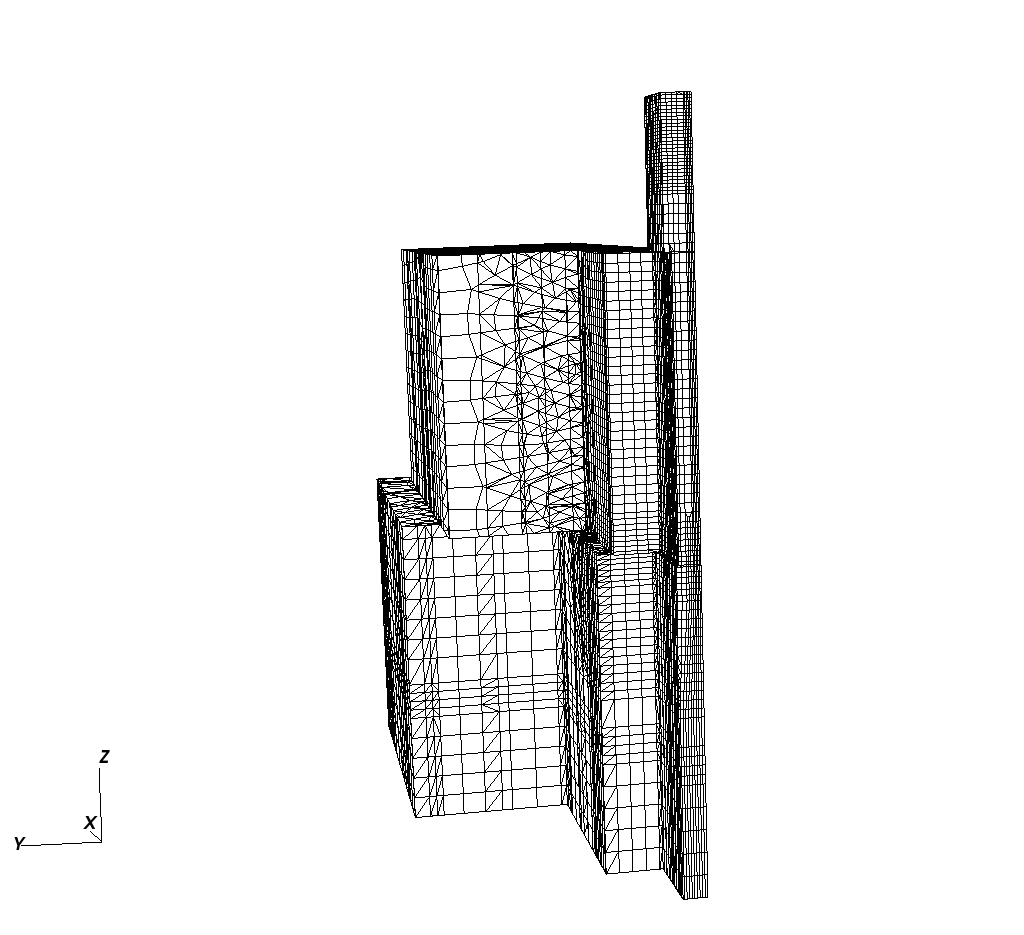
\includegraphics[trim={0cm 1cm 0cm 3cm},clip,scale=0.23]{../../figures/im1_foam_448.png}
\end{frame}
%%%%%%%%%%%%%%%%%%%%%%%%%%%%%%%%%%%%%%%%%%%%%%%%%%%%%%%%%%%%%%%%%%

\begin{frame}[t]\frametitle{Consequences of Load Balancing By Dimension}
  \begin{block}{}
  \begin{itemize}
    \item Perfect load balance in some cases will come at the cost of optimal sweeping (as shown in the next few slides).
    \item Time to solution is the most pertinent parameter, and if keeping a more optimal sweeping grid means a less balanced problem, then so be it.
    \item With imbalanced partitions it is harder to characterize the idle time, or the time where a processor has no work to do, and thus obtain an accurate stage count.
    \item A time-to-solution estimator must be built to more accurately predict sweep time.
  \end{itemize}
  \end{block}
\end{frame}
%%%%%%%%%%%%%%%%%%%%%%%%%%%%%%%%%%%%%%%%%%%%%%%%%%%%%%%%%%%%%%%%%%



\begin{frame}[t]\frametitle{Sweep on Regular Grid with 3 Angle Sets}
    \centering
	\animategraphics[loop,controls,width=0.7\linewidth]{10}{../../figures/sweeps_png/sweep_regular_20x20_as3_dog/sweep_regular_20x20_as3_dog_}{1}{48}
	%\href{run:figures/sweep_figs/sweeps_png/sweep_regular_20x20_as3_dog/animation.gif}{Animation.gif}
\end{frame}
%%%%%%%%%%%%%%%%%%%%%%%%%%%%%%%%%%%%%%%%%%%%%%%%%%%%%%%%%%%%%%%%%%

\begin{frame}[t]\frametitle{Sweep on LBD Grid with 3 Angle Sets}
   \centering
	\animategraphics[loop,controls,width=0.7\linewidth]{10}{../../figures/sweeps_png/sweep_random_20x20_as3_dog/sweep_random_20x20_as3_dog_}{1}{101}
	%\href{run:figures/sweep_figs/sweeps_png/sweep_random_20x20_as3_dog/animation.gif}{Animation.gif}
\end{frame}
%%%%%%%%%%%%%%%%%%%%%%%%%%%%%%%%%%%%%%%%%%%%%%%%%%%%%%%%%%%%%%%%%%


\begin{frame}[t]\frametitle{Sweep on Worst Grid with 1 Angle Set}
    \centering
	\animategraphics[loop,controls,width=0.7\linewidth]{10}{../../figures/sweeps_png/sweep_worst_20x20_as1_dog/sweep_worst_20x20_as1_dog_}{1}{230}
	%\href{run:figures/sweep_figs/sweeps_png/sweep_worst_20x20_as1_dog/animation.gif}{Animation.gif}
\end{frame}
%%%%%%%%%%%%%%%%%%%%%%%%%%%%%%%%%%%%%%%%%%%%%%%%%%%%%%%%%%%%%%%%%%

\section{Ongoing Work}
\subsection{}
%%%%%%%%%%%%%%%%%%%%%%%%%%%%%%%%%%%%%%%%%%%%%%%%%%%%%%%%%%%%%%%%%%%%%%%%%%%%%%%%%%%%%%%
%%%%%%%%%%%%%%%%%%%%%%%%%%%%%%%%%%%%%%%%%%%%%%%%%%%%%%%%%%%%%%%%%%%%%%%%%%%%%%%%%%%%%%%
%%%%%%%%%%%%%%%%%%%%%%%%%%%%%%%%%%%%%%%%%%%%%%%%%%%%%%%%%%%%%%%%%%%%%%%%%%%%%%%%%%%%%%%
%\section{Time-To-Solution Estimator}
%\subsection{}
%%%%%%%%%%%%%%%%%%%%%%%%%%%%%%%%%%%%%%%%%%%%%%%%%%%%%%%%%%%%%%%%%%%%%%%%%%%%%%%%%%%%%%%%
%%%%%%%%%%%%%%%%%%%%%%%%%%%%%%%%%%%%%%%%%%%%%%%%%%%%%%%%%%%%%%%%%%%%%%%%%%%%%%%%%%%%%%%%
%%%%%%%%%%%%%%%%%%%%%%%%%%%%%%%%%%%%%%%%%%%%%%%%%%%%%%%%%%%%%%%%%%%%%%%%%%%%%%%%%%%%%%%%
%
%\begin{frame}[t]\frametitle{Overview}
%\begin{block}{}
%\begin{itemize}
%	\item We need to optimize the cut plane location not for balance, but for the best possible sweep time.
%	\item We must build a time-to-solution estimator that calculates the time to solution for a given cut line partitioning and mesh cell density.
%	\item The time to solution estimator will be fed into an optimizing function that minimizes the time to solution. The cut planes corresponding to the minimum time to solution are the optimal partitioning scheme.
%\end{itemize}
%\end{block}
%\begin{block}{IMPORTANT}
%The time-to-solution estimator is a graph-based method that uses graph algorithms that rely on an acyclic graph. The partitioning schemes used CANNOT induce cycles.
%\end{block}
%\end{frame}
%%%%%%%%%%%%%%%%%%%%%%%%%%%%%%%%%%%%%%%%%%%%%%%%%%%%%%%%%%%%%%%%%%
%
\begin{frame}[t]\frametitle{Time To Solution Estimator}
\begin{block}{}
\begin{enumerate}
    \item Given a partitioning scheme, build an adjacency matrix.
    \item From the adjacency matrix, build Directed Acyclic Graphs (DAGs), one for each quadrant/octant.
    \item Weight each DAG's edges based on the solve and communication time of each subset to its neighbors.
    \item Create a universal timescale and launch processes based on when graph predecessor has finished its work.
    \item When conflicts arise between octants, resolve with first-come/first-serve and adjust weights (time delays) of the losing graph nodes.
    \item Sweeping time is obtain at the conclusion of this process.
\end{enumerate}
\end{block}
Using this as performance model, we can evaluate the qualities of various parallel partitions for unstructured grids.

\vspace{2cm}
In the next slides, some details on items \#2-5.
\end{frame}
%%%%%%%%%%%%%%%%%%%%%%%%%%%%%%%%%%%%%%%%%%%%%%%%%%%%%%%%%%%%%%%%%%

\begin{frame}[t]\frametitle{Directed Acyclic Graphs (DAG)}
  \begin{columns}
  \column{0.5\textwidth}
    \centering
    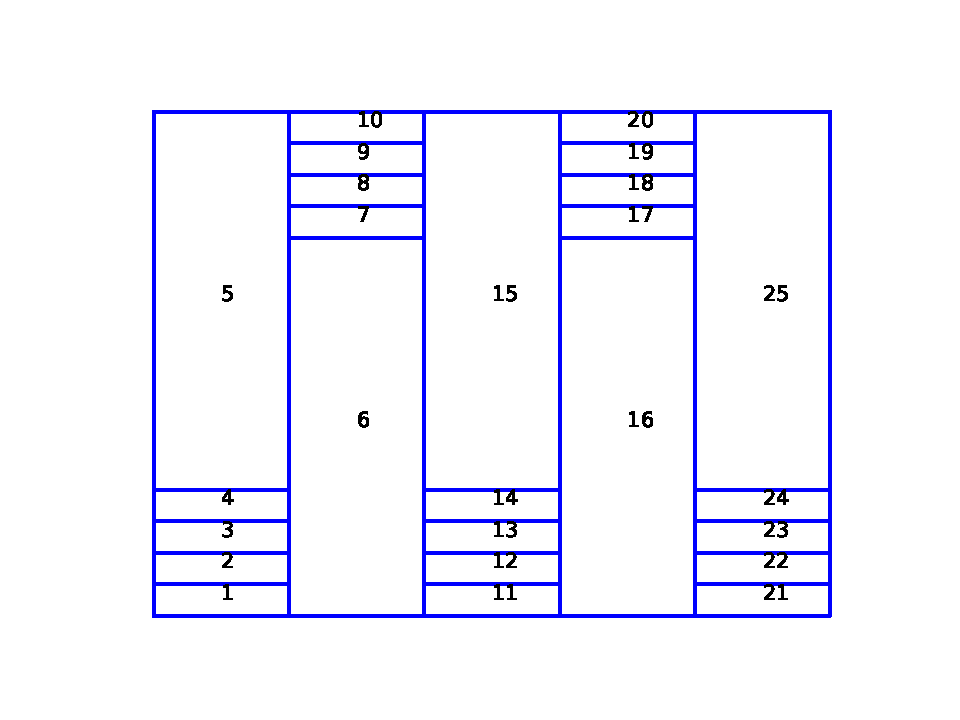
\includegraphics[scale=0.5]{../../figures/boundaries_worst_pres.pdf}
    \column{0.5\textwidth}
    \centering
    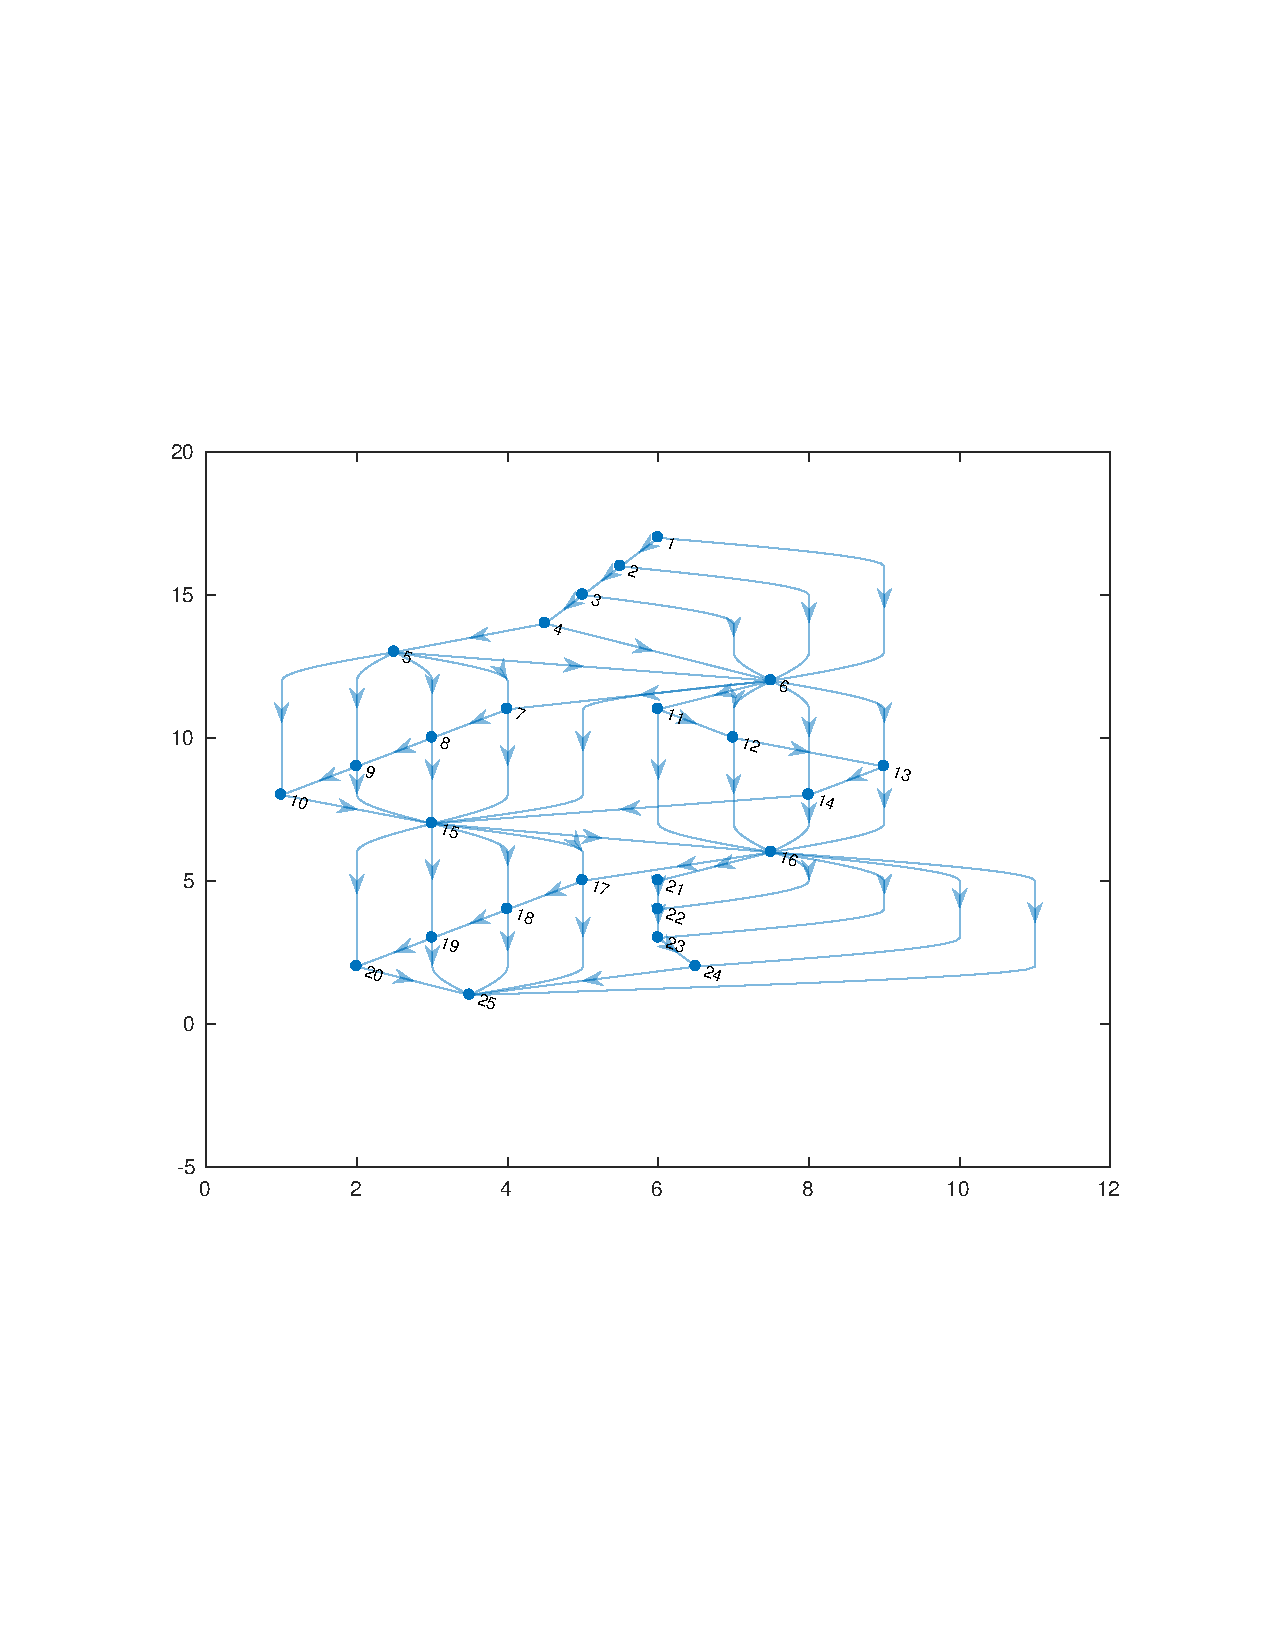
\includegraphics[scale=0.35,trim={0cm 0cm 0cm 5cm},clip]{../../figures/layered.pdf}
  \end{columns}
\end{frame}
%%%%%%%%%%%%%%%%%%%%%%%%%%%%%%%%%%%%%%%%%%%%%%%%%%%%%%%%%%%%%%%%%%
%
%\begin{frame}[t]\frametitle{Building the Adjacency Matrix}
%\begin{block}{}
%\begin{itemize}
%  \item The adjacency matrix provides the crucial connectivity information necessary to build the Task Dependence Graphs (TDG's) in the time-to-solution estimator.
%\end{itemize}
%\end{block}
%\begin{minipage}{0.49\textwidth}
%\centering
%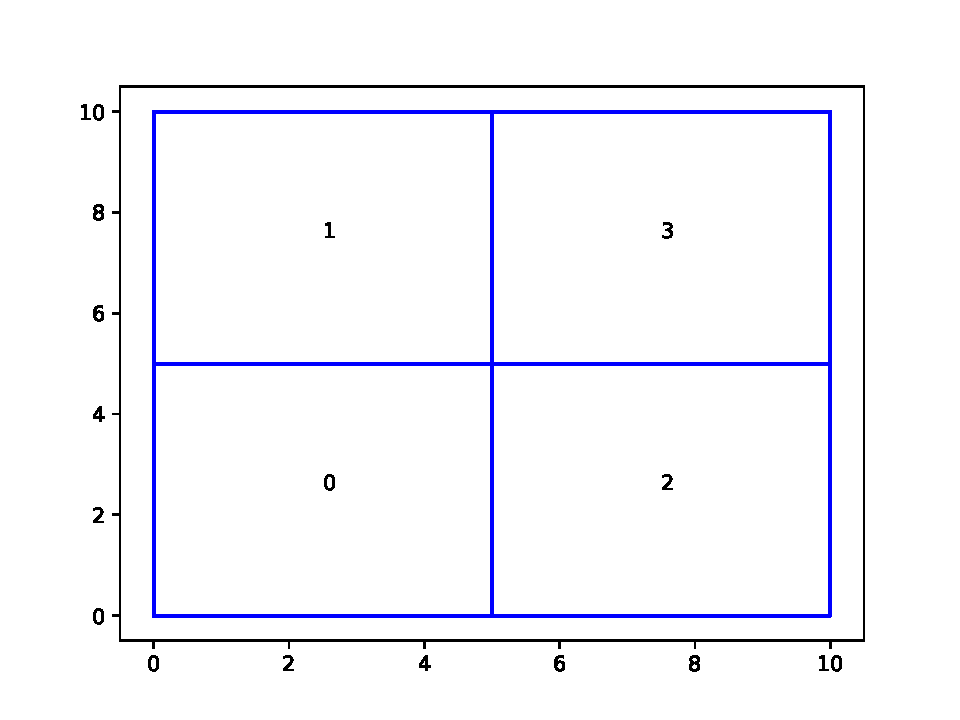
\includegraphics[scale=0.4]{../../figures/base_adjacency_layout.pdf}
%\end{minipage}
%\begin{minipage}{0.49\textwidth}
%\centering
%$\begin{pmatrix}
%0 & 1 & 1  & 0  \\
%1 & 0 & 0 & 1 \\
%1 & 0 & 0 & 1 \\ 
%0 & 1 & 1 & 0 \\
%\end{pmatrix}$
%\end{minipage}
%\end{frame}
%%%%%%%%%%%%%%%%%%%%%%%%%%%%%%%%%%%%%%%%%%%%%%%%%%%%%%%%%%%%%%%%%%
%
%\begin{frame}[t]\frametitle{Building the Task Dependence Graphs}
%\begin{block}{}
%\begin{itemize}
%    \item Each quadrant/octant gets its own TDG.
%    \item The opposing quadrant/octant pairs have opposing sweep orderings. 
%    \item Each set of quadrant/octant pairs uses a different adjacency matrix. 
%    \item Python package \textbf{networkx} is used for all graph operations.
%\end{itemize}
%\end{block}
%\centering
%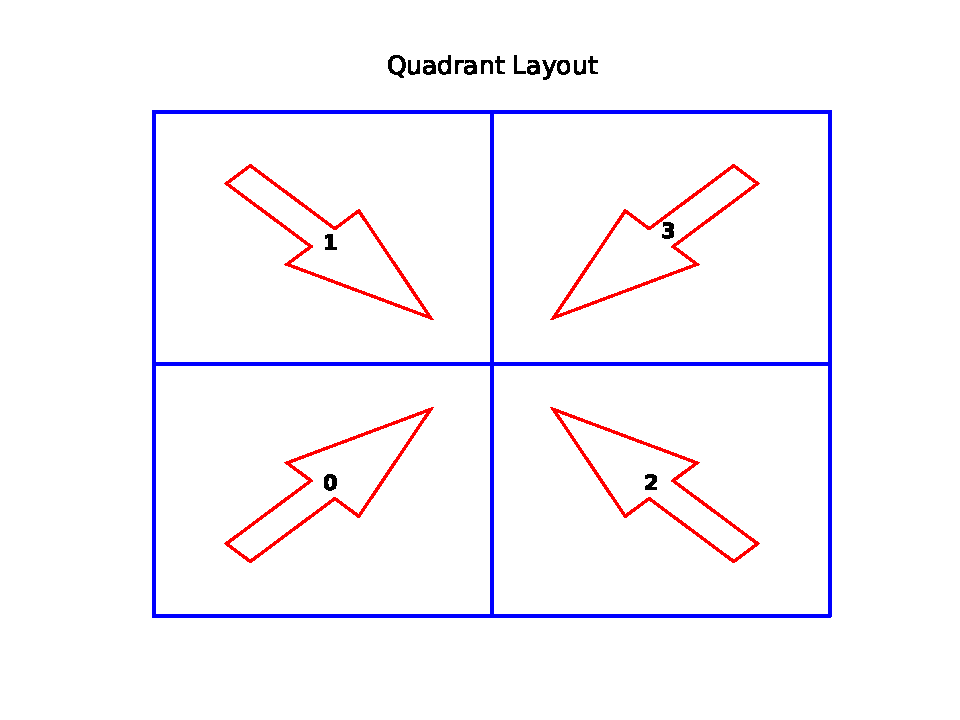
\includegraphics[scale=0.45]{../../figures/quadrant_layout.pdf}
%\end{frame}
%%%%%%%%%%%%%%%%%%%%%%%%%%%%%%%%%%%%%%%%%%%%%%%%%%%%%%%%%%%%%%%%%%
%
%\begin{frame}[t]\frametitle{Quadrants 0 and 3}
%\begin{block}{}
%\begin{itemize}
%    \item We use the upper triangular portion of the adjacency matrix for quadrant 0.
%    \item We use the lower triangular portion of the adjacency matrix for quadrant 3.
%\end{itemize}
%\end{block}
%\begin{minipage}{0.49\textwidth}
%  \centering
%  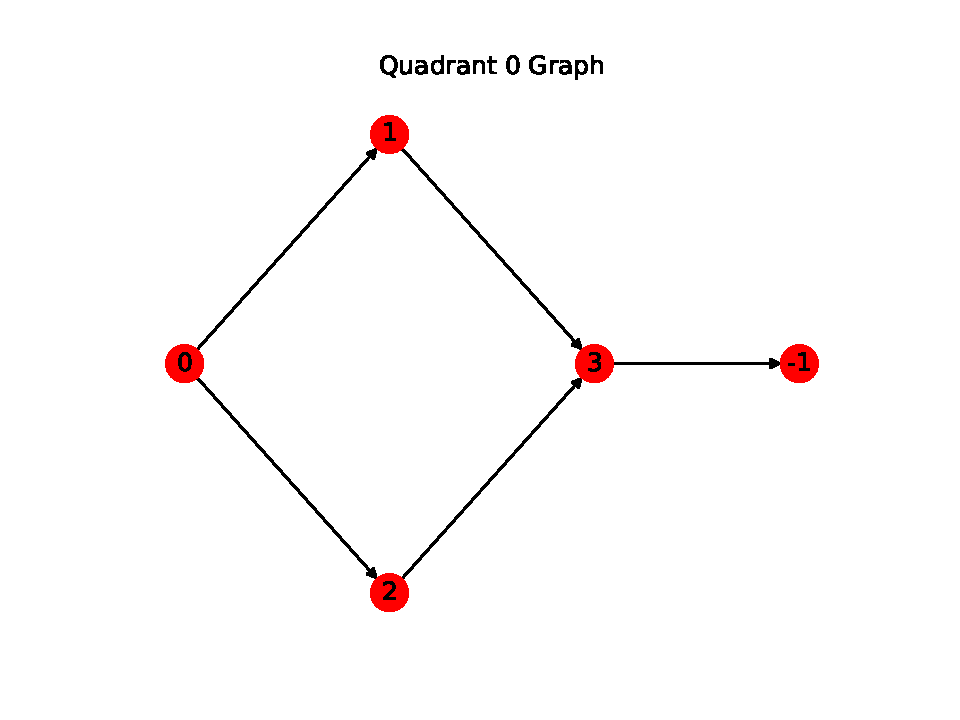
\includegraphics[scale=0.35]{../../figures/q0_preweight.pdf}
%\end{minipage}
%\begin{minipage}{0.49\textwidth}
%  \centering
%  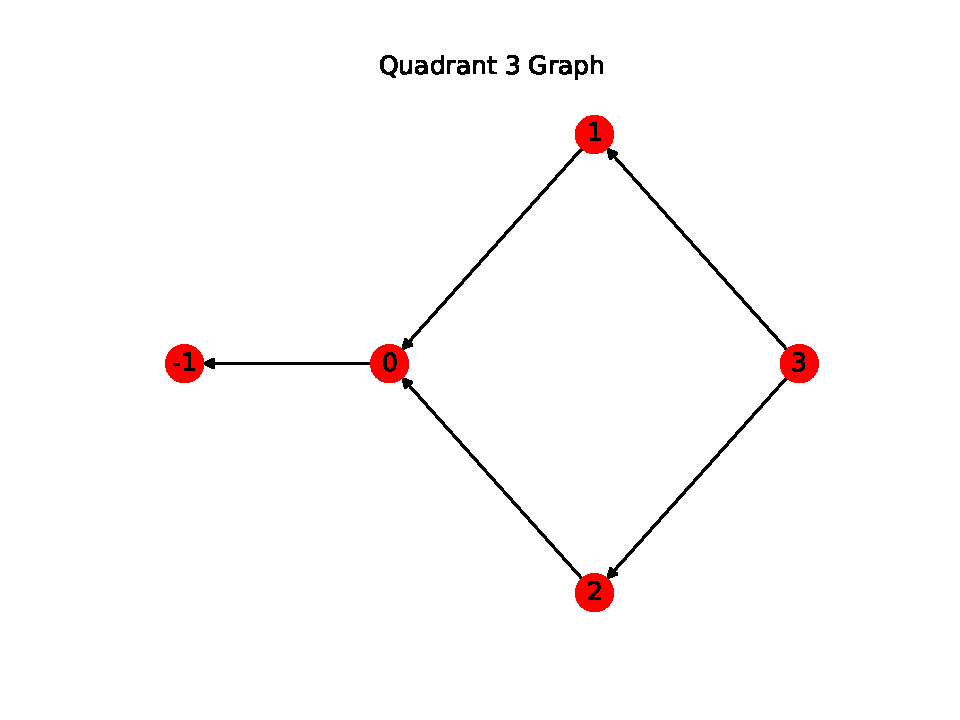
\includegraphics[scale=0.35]{../../figures/q3_preweight.pdf}
%\end{minipage}
%\end{frame}
%%%%%%%%%%%%%%%%%%%%%%%%%%%%%%%%%%%%%%%%%%%%%%%%%%%%%%%%%%%%%%%%%%
%
%\begin{frame}[t]\frametitle{Quadrants 1 and 2}
%  \begin{block}{}
%    \begin{itemize}
%      \item Before building the graphs for these opposing quadrants, we have to alter the adjacency matrix slightly.
%      \item The subsets get renumbered in a manner where subset 1 becomes subset 0, subset 0 becomes subset 1, etc. In short the column numbering is flipped, and a ``flipped'' adjacency matrix is built. 
%    \end{itemize}
%  \end{block}
%  \begin{minipage}{0.49\textwidth}
%    \centering
%    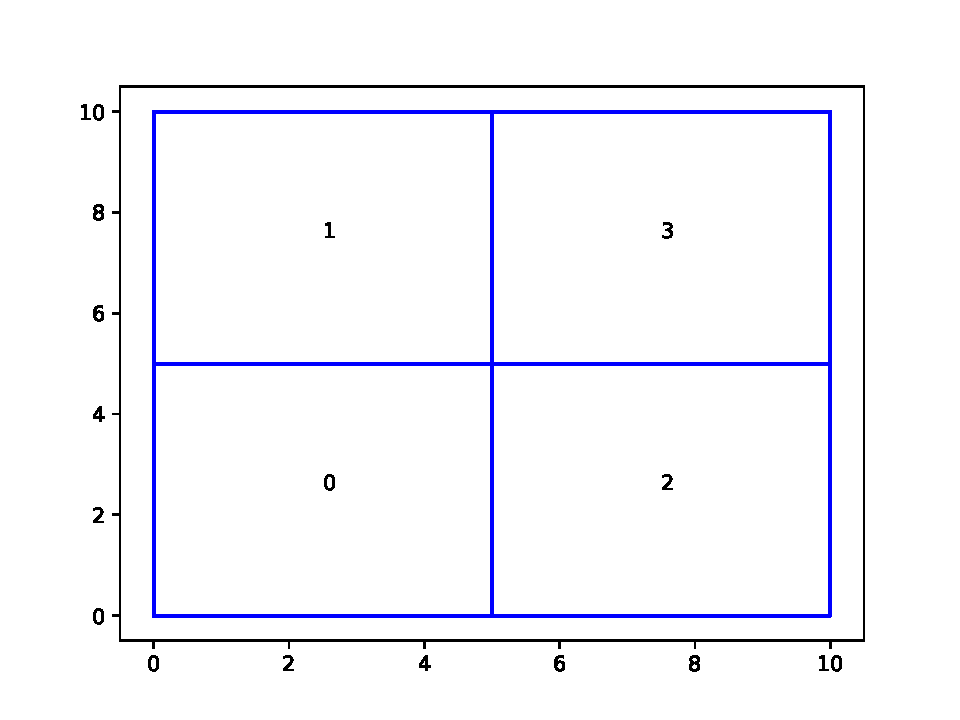
\includegraphics[scale=0.38]{../../figures/base_adjacency_layout.pdf}
%  \end{minipage}
%  \begin{minipage}{0.49\textwidth}
%    \centering
%    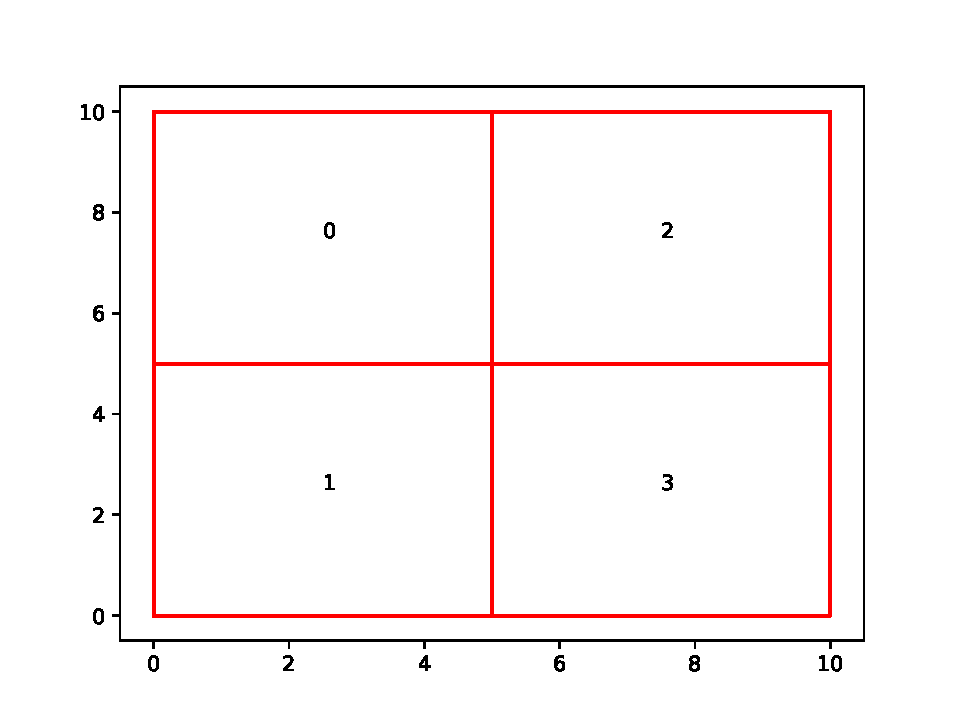
\includegraphics[scale=0.38]{../../figures/flipped_subset_layout.pdf}
%  \end{minipage}
%\end{frame}
%%%%%%%%%%%%%%%%%%%%%%%%%%%%%%%%%%%%%%%%%%%%%%%%%%%%%%%%%%%%%%%%%%
%
%\begin{frame}[t]\frametitle{Quadrants 1 and 2}
%  \begin{block}{}
%    \begin{itemize}
%      \item We use the upper triangular portion of the ``flipped'' adjacency matrix for quadrant 1.
%      \item We use the lower triangular portion of the ``flipped'' adjacency matrix for quadrant 2.
%    \end{itemize}
%  \end{block}
%  \begin{minipage}{0.49\textwidth}
%    \centering
%    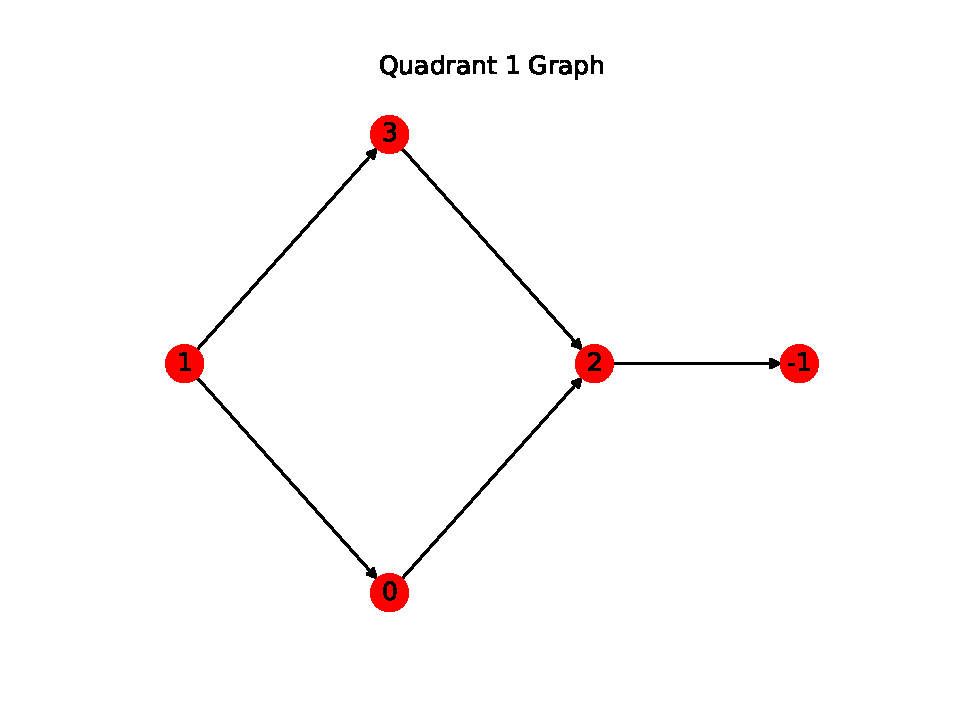
\includegraphics[scale=0.35]{../../figures/q1_preweight.pdf}
%  \end{minipage}
%  \begin{minipage}{0.49\textwidth}
%    \centering
%    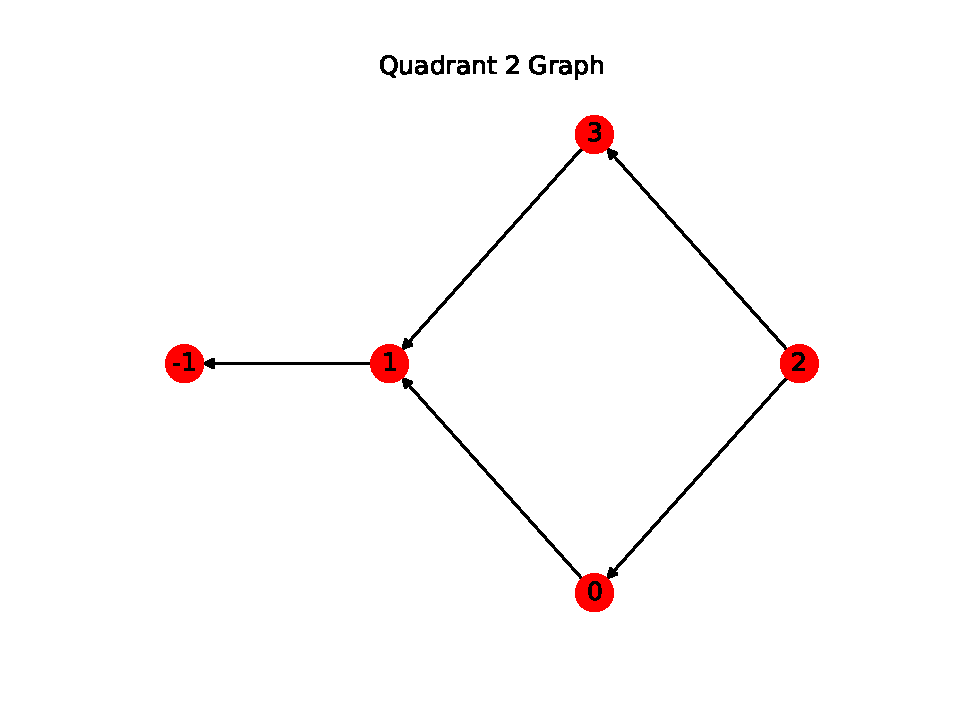
\includegraphics[scale=0.35]{../../figures/q2_preweight.pdf}
%  \end{minipage}
%\end{frame}
%%%%%%%%%%%%%%%%%%%%%%%%%%%%%%%%%%%%%%%%%%%%%%%%%%%%%%%%%%%%%%%%%%
%
\begin{frame}[t]\frametitle{Weighting the TDGs}
  \begin{block}{}
    \begin{itemize}
    \item Graph edge weight = time to solve cells in subset \& communicate boundary values to downwind subsets.
    \begin{align}
      \text{weight} = T_{wu} + N_c\cdot (T_c+ A_m\cdot(T_m + T_g)) + N_{b}\cdot A_m\cdot T_{\text{comm}} + \text{latency}\\
      \end{align}
    \begin{footnotesize}
    \begin{equation*}
    \begin{aligned}[c]
    N_c &= \text{number of cells}  \\
    A_m &= \text{Number of angles per task}  \\
    T_c &= \text{Time spent on cell-specific work}  \\
    T_{\text{comm}} &= \text{Comm time per double} \\ 
    \end{aligned}
    \begin{aligned}[c]
     N_b &=(\text{num boundary cells})\cdot \text{boundary unknowns per cell} \\
     T_m &= \text{Time spent on angle-specific work} \\
     T_g &= \text{Time spend on group-specific work} \\
     T_{wu} &= \text{Time to get into sweep operator} \\
     \end{aligned}
    \end{equation*}
    \end{footnotesize}
    \end{itemize}
  \end{block}

For unstructured grids, we use a mesh density function to calculate the \# cells per subset and \# of boundary cells. \\
\vspace{1cm}
In practice, we use mesh cell centroids to build a discrete mesh density function.
%    	\item The weight of the edge between two nodes (subsets) in the graph represents the solve and communication time of the base node.
%  \begin{block}{}
%    \begin{align}
%    \text{cells per subset} &= \int_{\tcr{x_i}}^{\tcr{x_{i+1}}} \int_{\tcr{y_j}}^{\tcr{y_{j+1}}} \int_{\tcr{z_k}}^{\tcr{z_{k+1}}} \text{mesh density } dx dy dz \\
%    \label{weight}
%      \text{weight} &= T_{wu} + N_c\cdot (T_c+ A_m\cdot(T_m + T_g)) + N_{b}\cdot A_m\cdot T_{\text{comm}} + \text{latency}\\
%      \end{align}
%    \footnotesize
%    \begin{equation*}
%    \begin{aligned}[c]
%    N_c &= \text{number of cells}  \\
%    A_m &= \text{Number of angles per task}  \\
%    T_c &= \text{Time spent on cell-specific work}  \\
%    T_{\text{comm}} &= \text{Comm time per double} \\ 
%    \end{aligned}
%    \begin{aligned}[c]
%     N_b &\approx(\text{num boundary cells})\cdot \text{boundary unknowns per cell} \\
%     T_m &= \text{Time spent on angle-specific work} \\
%     T_g &= \text{Time spend on group-specific work} \\
%     T_{wu} &= \text{Time to get into sweep operator} \\
%     \end{aligned}
%    \end{equation*}
%  \end{block}
\end{frame}
%%%%%%%%%%%%%%%%%%%%%%%%%%%%%%%%%%%%%%%%%%%%%%%%%%%%%%%%%%%%%%%%%%
%
%\begin{frame}[t]\frametitle{Weighting the TDGs}
%  \begin{minipage}{0.49\textwidth}
%    \centering
%    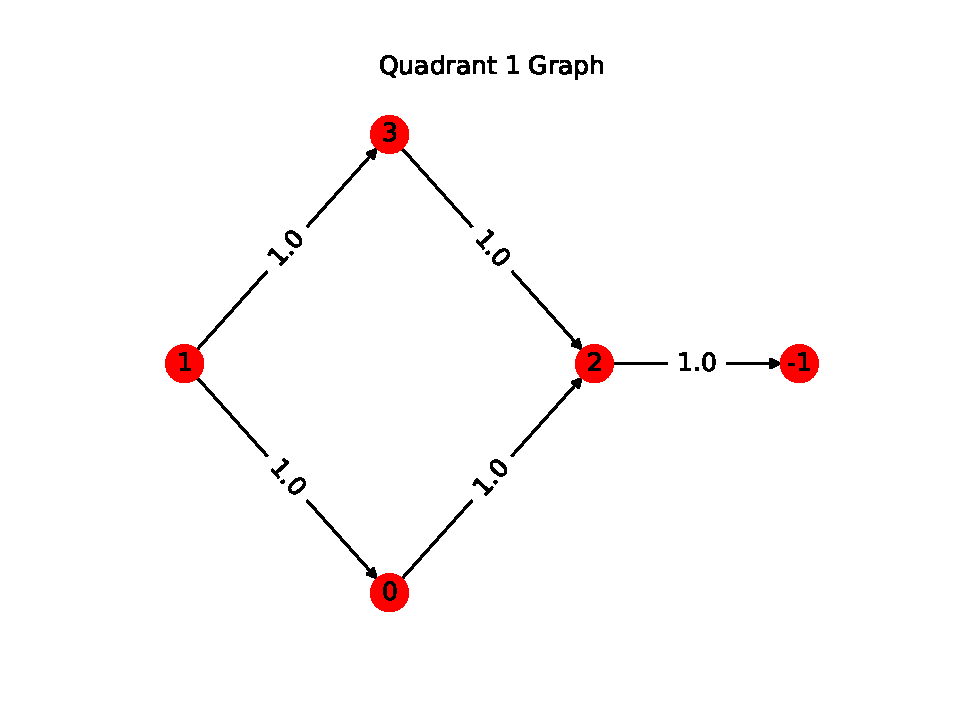
\includegraphics[scale=0.32]{../../figures/q1_postweight.pdf}
%  \end{minipage}
%  \begin{minipage}{0.49\textwidth}
%    \centering
%    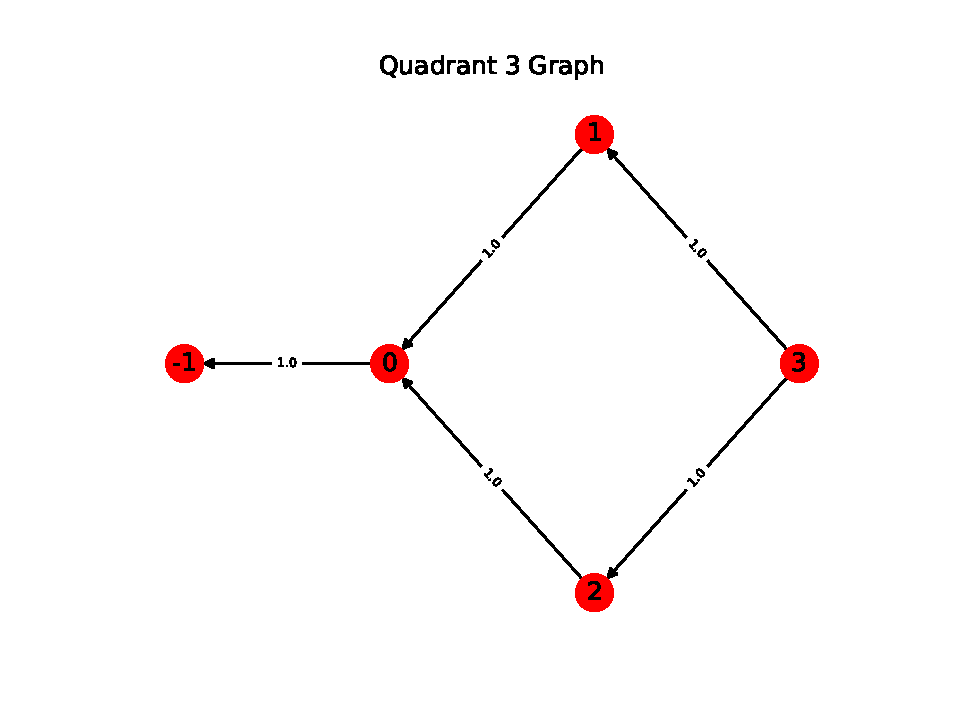
\includegraphics[scale=0.32]{../../figures/q3_postweight.pdf}
%  \end{minipage}
%  \begin{minipage}{0.49\textwidth}
%    \centering
%    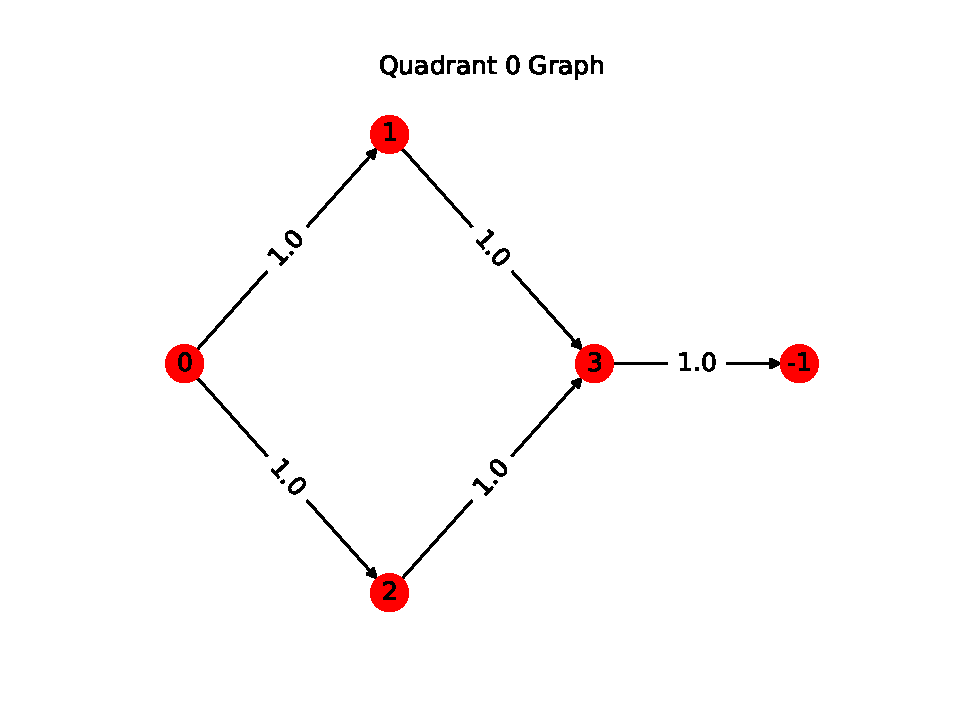
\includegraphics[scale=0.32]{../../figures/q0_postweight.pdf}
%  \end{minipage}
%  \begin{minipage}{0.49\textwidth}
%    \centering
%    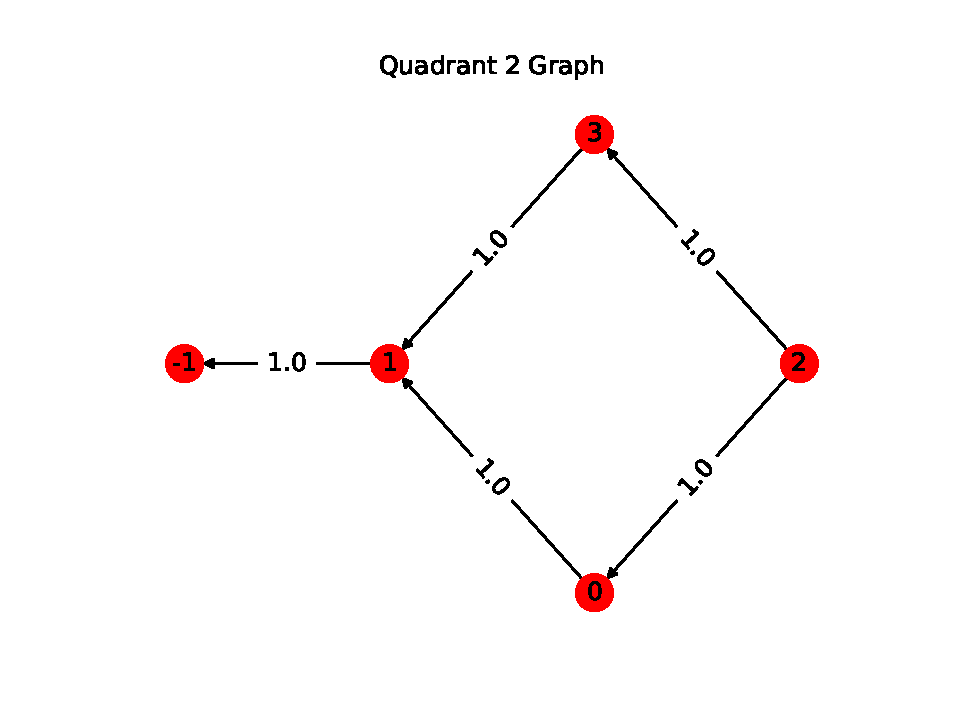
\includegraphics[scale=0.32]{../../figures/q2_postweight.pdf}
%  \end{minipage}
% 
%\end{frame}
%%%%%%%%%%%%%%%%%%%%%%%%%%%%%%%%%%%%%%%%%%%%%%%%%%%%%%%%%%%%%%%%%%
%
%\begin{frame}[t]\frametitle{Adjusting for Multiple Angles}
% \begin{minipage}{0.49\textwidth}
%    \centering
%    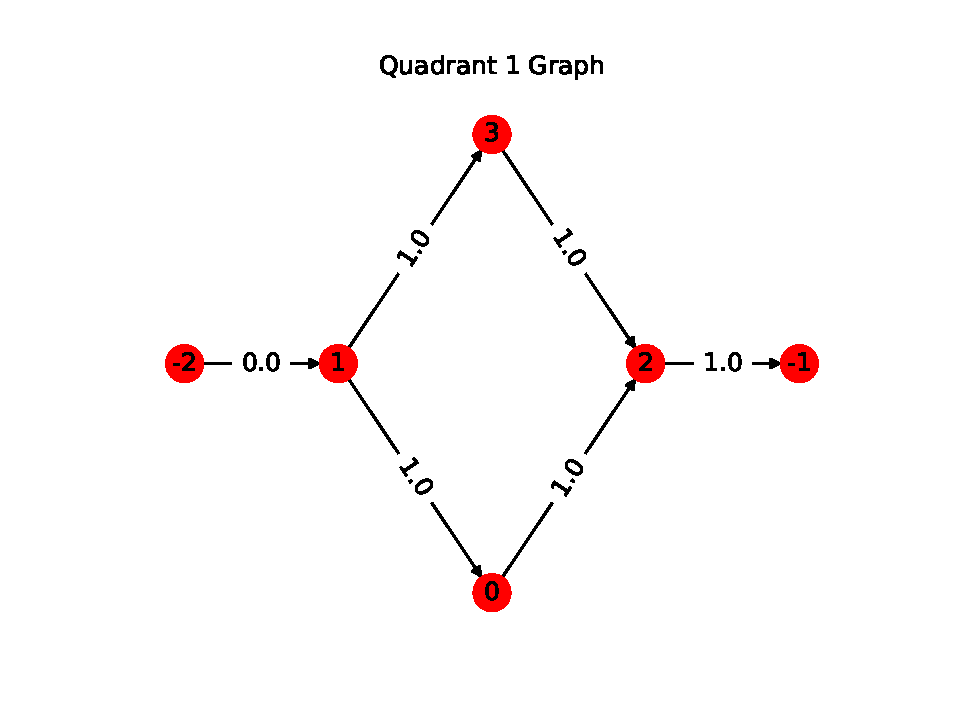
\includegraphics[scale=0.32]{../../figures/q1_postpipeline.pdf}
%  \end{minipage}
%  \begin{minipage}{0.49\textwidth}
%    \centering
%    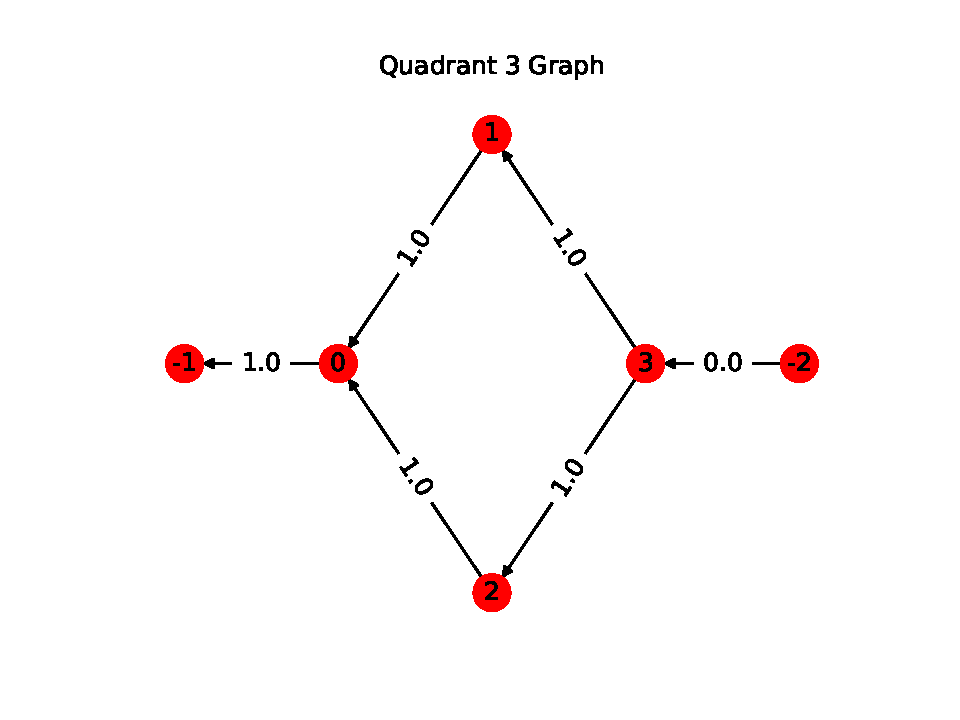
\includegraphics[scale=0.32]{../../figures/q3_postpipeline.pdf}
%  \end{minipage}
%  \begin{minipage}{0.49\textwidth}
%    \centering
%    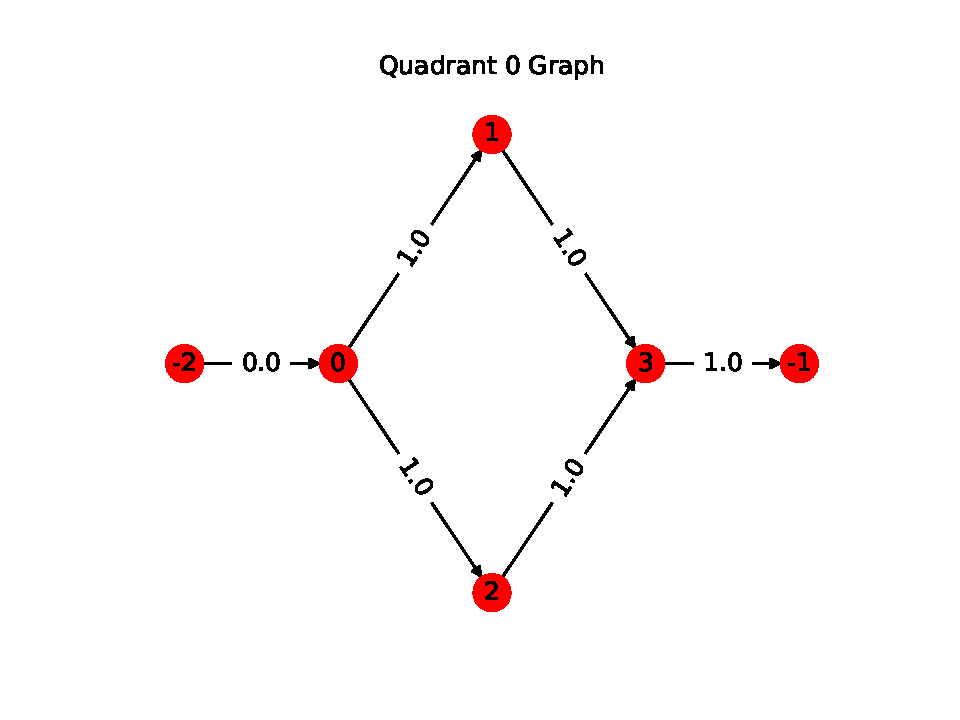
\includegraphics[scale=0.32]{../../figures/q0_postpipeline.pdf}
%  \end{minipage}
%  \begin{minipage}{0.49\textwidth}
%    \centering
%    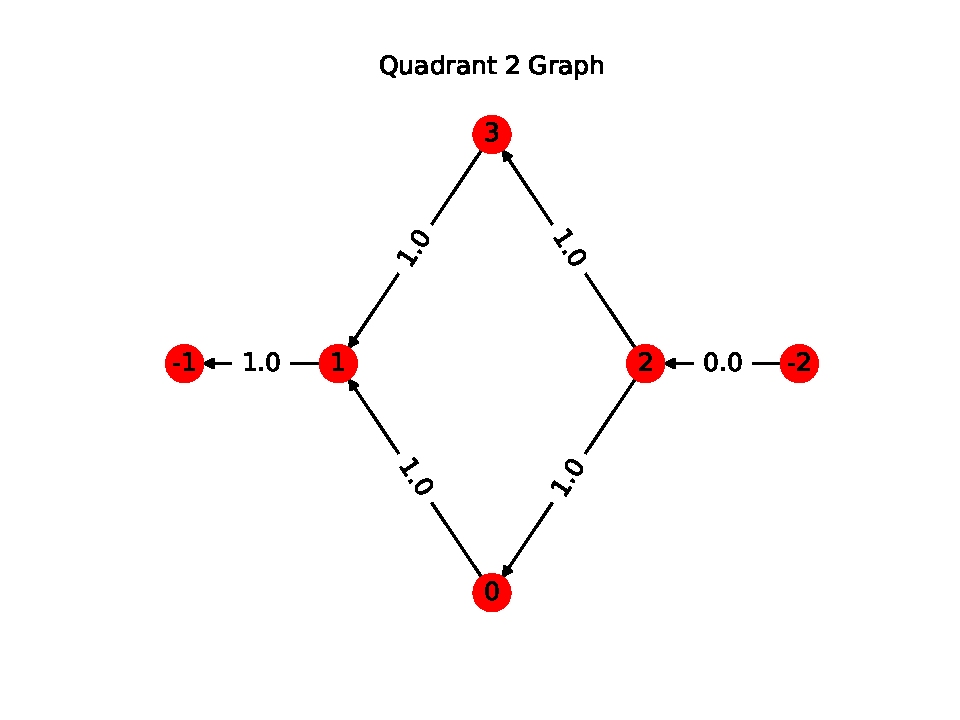
\includegraphics[scale=0.32]{../../figures/q2_postpipeline.pdf}
%  \end{minipage}
%\end{frame}
%%%%%%%%%%%%%%%%%%%%%%%%%%%%%%%%%%%%%%%%%%%%%%%%%%%%%%%%%%%%%%%%%%
%
%\begin{frame}[t]\frametitle{Second Angleset}
% \begin{minipage}{0.49\textwidth}
%    \centering
%    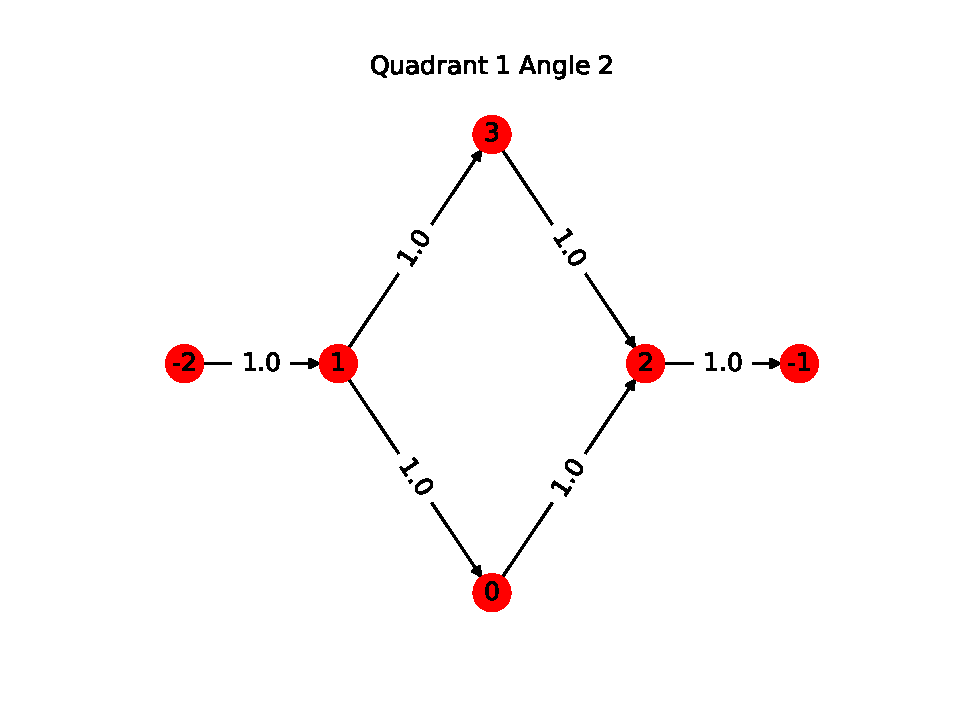
\includegraphics[scale=0.32]{../../figures/q5_postpipeline.pdf}
%  \end{minipage}
%  \begin{minipage}{0.49\textwidth}
%    \centering
%    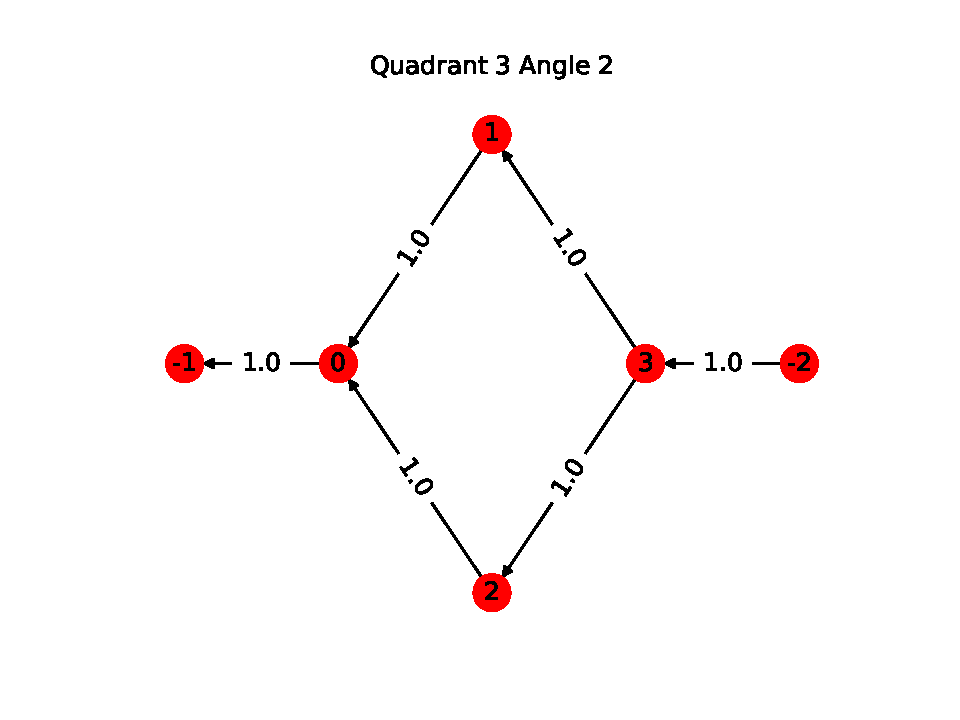
\includegraphics[scale=0.32]{../../figures/q7_postpipeline.pdf}
%  \end{minipage}
%  \begin{minipage}{0.49\textwidth}
%    \centering
%    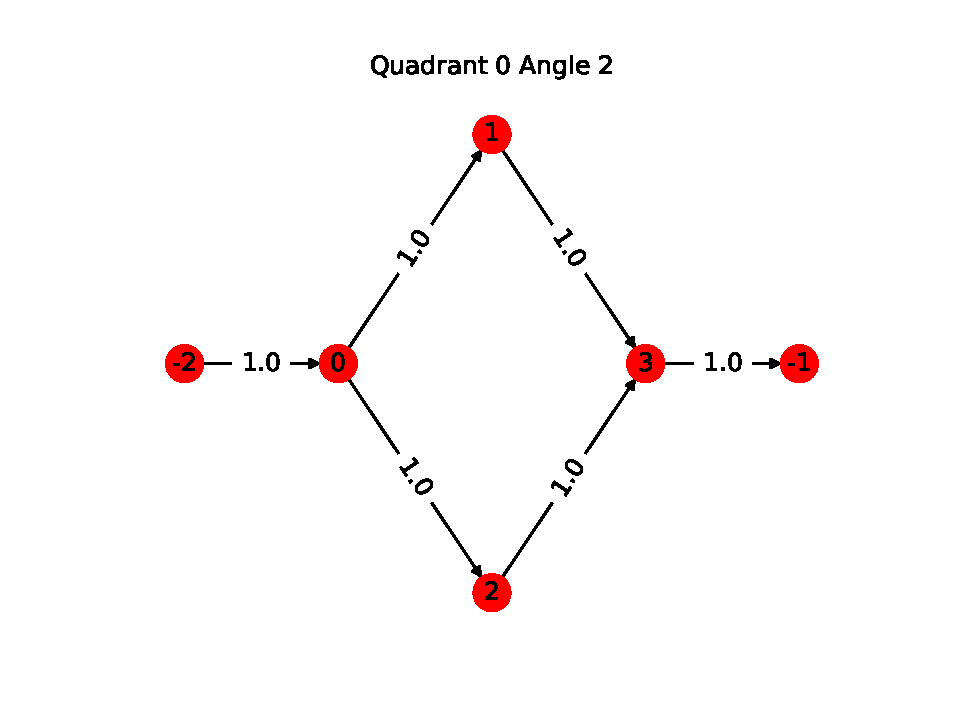
\includegraphics[scale=0.32]{../../figures/q4_postpipeline.pdf}
%  \end{minipage}
%  \begin{minipage}{0.49\textwidth}
%    \centering
%    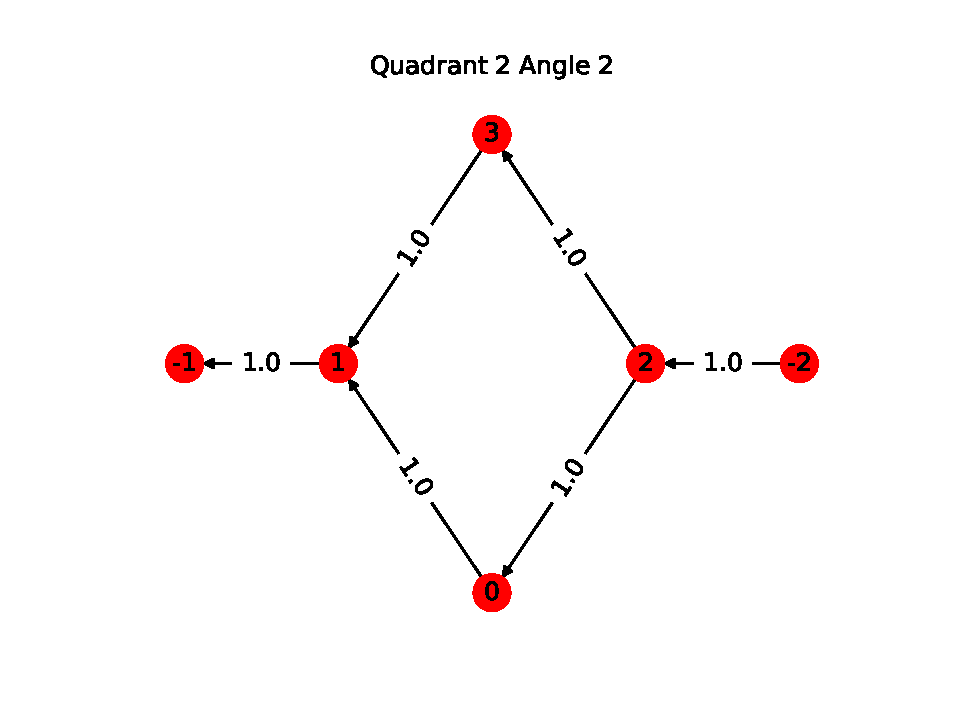
\includegraphics[scale=0.32]{../../figures/q6_postpipeline.pdf}
%  \end{minipage}
%\end{frame}
%%%%%%%%%%%%%%%%%%%%%%%%%%%%%%%%%%%%%%%%%%%%%%%%%%%%%%%%%%%%%%%%%%
%
\begin{frame}[t]\frametitle{Universal Edge Weighting}
  \begin{block}{}
    \begin{itemize}
      \item Once the weight (solve + comm. time) for each edge are known, the next step is to order them on a universal time scale. 
      \item To do this, we calculate the sum of the longest weighted path to each node, and set all incoming edges to each node to this value.
%      \item To find the longest weighted path, the graph weights are inverted, and the shortest weighted path is found. The original edge weights are used to calculate the value of the longest weighted path.
      \item The resulting graph is thus weighted so that the incoming edge to each node represents the time at which that node is ready to solve.
    \end{itemize}
  \end{block}
\end{frame}
%%%%%%%%%%%%%%%%%%%%%%%%%%%%%%%%%%%%%%%%%%%%%%%%%%%%%%%%%%%%%%%%%%
%\begin{frame}[t]\frametitle{Universal Edge Weighting}
% \begin{minipage}{0.49\textwidth}
%    \centering
%    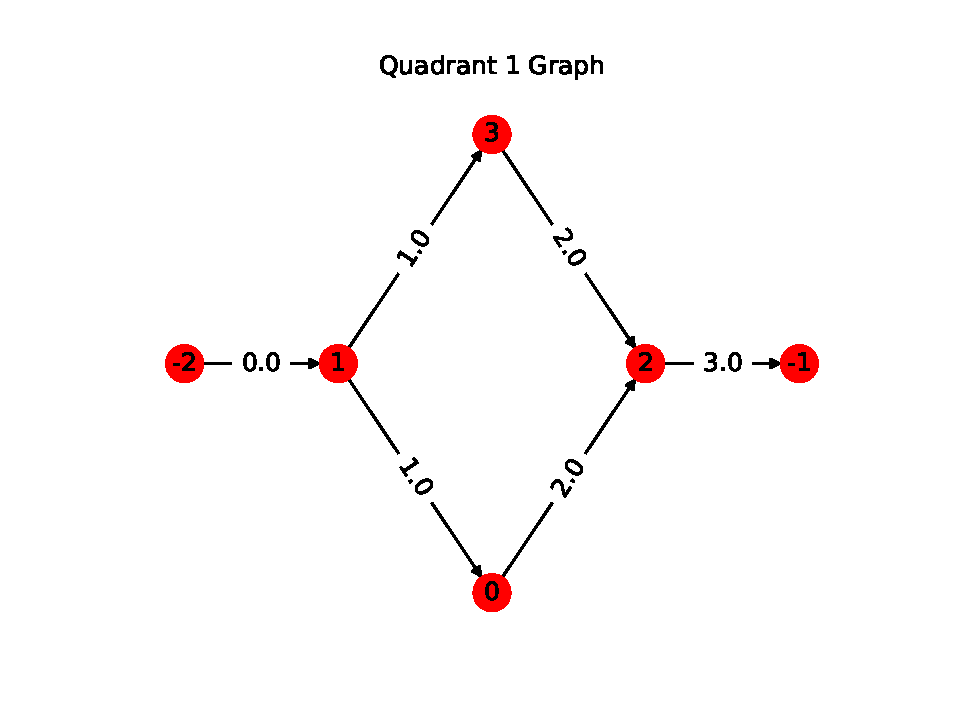
\includegraphics[scale=0.32]{../../figures/q1_postuniversal.pdf}
%  \end{minipage}
%  \begin{minipage}{0.49\textwidth}
%    \centering
%    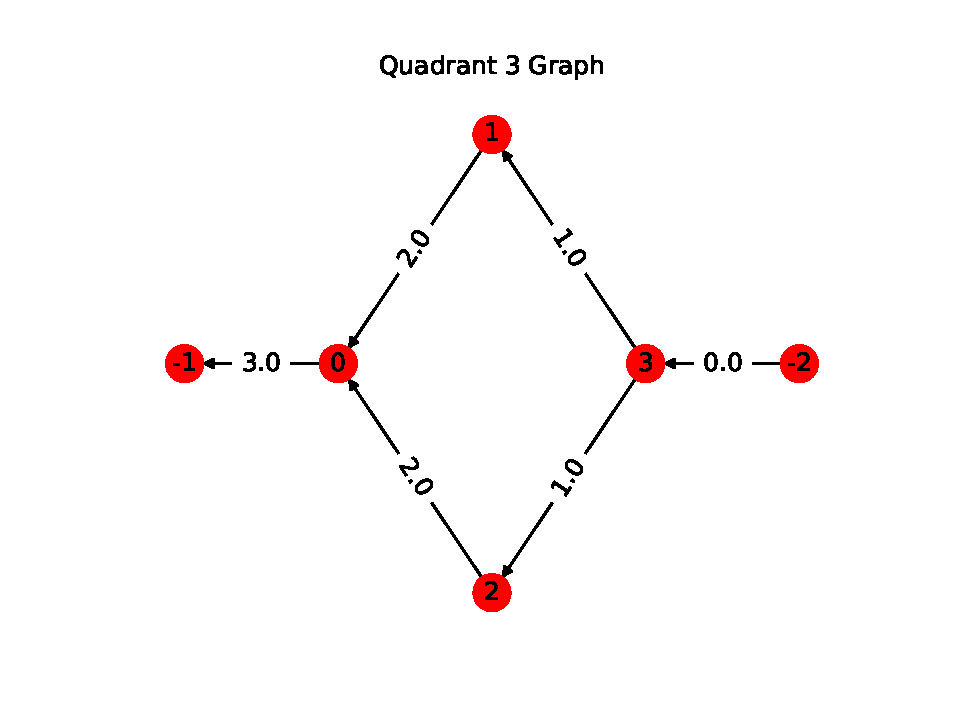
\includegraphics[scale=0.32]{../../figures/q3_postuniversal.pdf}
%  \end{minipage}
%  \begin{minipage}{0.49\textwidth}
%    \centering
%    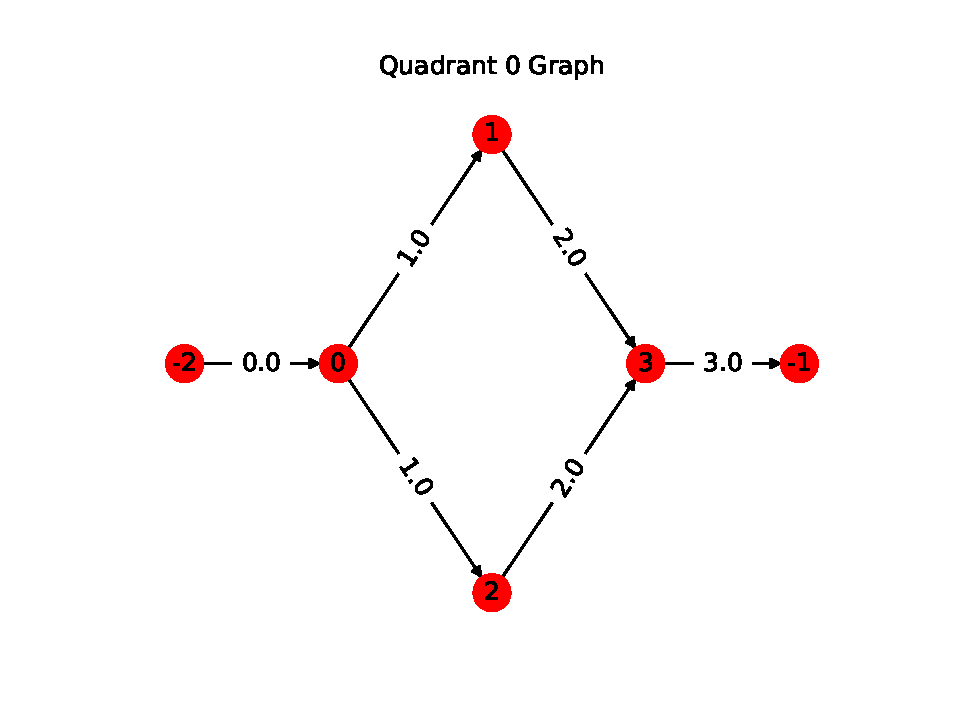
\includegraphics[scale=0.32]{../../figures/q0_postuniversal.pdf}
%  \end{minipage}
%  \begin{minipage}{0.49\textwidth}
%    \centering
%    \includegraphics[scale=0.32]{../../figures/q2_postuniversal.pdf}
%  \end{minipage}
%\end{frame}
%%%%%%%%%%%%%%%%%%%%%%%%%%%%%%%%%%%%%%%%%%%%%%%%%%%%%%%%%%%%%%%%%%
%
%\begin{frame}[t]\frametitle{Second Angleset}
% \begin{minipage}{0.49\textwidth}
%    \centering
%    \includegraphics[scale=0.32]{../../figures/q5_postuniversal.pdf}
%  \end{minipage}
%  \begin{minipage}{0.49\textwidth}
%    \centering
%    \includegraphics[scale=0.32]{../../figures/q7_postuniversal.pdf}
%  \end{minipage}
%  \begin{minipage}{0.49\textwidth}
%    \centering
%    \includegraphics[scale=0.32]{../../figures/q4_postuniversal.pdf}
%  \end{minipage}
%  \begin{minipage}{0.49\textwidth}
%    \centering
%    \includegraphics[scale=0.32]{../../figures/q6_postuniversal.pdf}
%  \end{minipage}
%\end{frame}
%%%%%%%%%%%%%%%%%%%%%%%%%%%%%%%%%%%%%%%%%%%%%%%%%%%%%%%%%%%%%%%%%%
%
%\begin{frame}[t]\frametitle{Conflict Detection and Resolution}
%  \begin{block}{}
%    \begin{itemize}
%      \item Best summarized as a ``marching" process. 
%      \item Starting at time $t=0$, find the first interaction (recalling that the incoming weight to a node reflects the time it is ready to solve).
%      \item If at time $t$, multiple TDGs are solving the same node, this means there is a conflict. 
%      \item  ``Losing" TDGs modify their downstream weights according to how long they are delayed.
%    \end{itemize}
%  \end{block}
%\end{frame}
%%%%%%%%%%%%%%%%%%%%%%%%%%%%%%%%%%%%%%%%%%%%%%%%%%%%%%%%%%%%%%%%%%
%
\begin{frame}[t]\frametitle{First Come First Serve Conflict Resolution}
\begin{block}{}
\begin{itemize}
	\item The first octant to arrive to a graph node will begin solving it, and the remaining octants will incur a delay (if applicable).
	\item The delay is reflected in each remaining Task-Dependent Graph by adding the corresponding delay as a weight to the applicable edge and applicable downstream edges.
  \item If two octants arrive to a node at exactly the same time, the octant with the greater remaining depth-of-graph and priority-octant wins the tie.
\end{itemize}
\end{block}
  \begin{block}{Unweighted vs. Weighted Depth-of-Graph Remaining}
    \begin{itemize}
      \item There are two options for the depth-of-graph remaining. Unweighted does not take the weights into account, and weighted looks at the final time for the conflicting graphs on the universal time scale.
    \end{itemize}
  \end{block}
\end{frame}
%%%%%%%%%%%%%%%%%%%%%%%%%%%%%%%%%%%%%%%%%%%%%%%%%%%%%%%%%%%%%%%%%%
%
%\begin{frame}[t]\frametitle{$t=1$: Graphs 0,3 and Graphs 1,2 in Conflict}
% \begin{minipage}{0.49\textwidth}
%    \centering
%    \includegraphics[scale=0.32]{../../figures/graph_1_0_1.pdf}
%  \end{minipage}
%  \begin{minipage}{0.49\textwidth}
%    \centering
%    \includegraphics[scale=0.32]{../../figures/graph_1_0_3.pdf}
%  \end{minipage}
%  \begin{minipage}{0.49\textwidth}
%    \centering
%    \includegraphics[scale=0.32]{../../figures/graph_1_0_0.pdf}
%  \end{minipage}
%  \begin{minipage}{0.49\textwidth}
%    \centering
%    \includegraphics[scale=0.32]{../../figures/graph_1_0_2.pdf}
%  \end{minipage}
%\end{frame}
%%%%%%%%%%%%%%%%%%%%%%%%%%%%%%%%%%%%%%%%%%%%%%%%%%%%%%%%%%%%%%%%%%
%
%\begin{frame}[t]\frametitle{$t=2$: Graphs 0 and 1 Won, Still in Conflict}
% \begin{minipage}{0.49\textwidth}
%    \centering
%    \includegraphics[scale=0.32]{../../figures/graph_2_1_1.pdf}
%  \end{minipage}
%  \begin{minipage}{0.49\textwidth}
%    \centering
%    \includegraphics[scale=0.32]{../../figures/graph_2_1_3.pdf}
%  \end{minipage}
%  \begin{minipage}{0.49\textwidth}
%    \centering
%    \includegraphics[scale=0.32]{../../figures/graph_2_1_0.pdf}
%  \end{minipage}
%  \begin{minipage}{0.49\textwidth}
%    \centering
%    \includegraphics[scale=0.32]{../../figures/graph_2_1_2.pdf}
%  \end{minipage}
%\end{frame}
%%%%%%%%%%%%%%%%%%%%%%%%%%%%%%%%%%%%%%%%%%%%%%%%%%%%%%%%%%%%%%%%%%
%
%\begin{frame}[t]\frametitle{$t=3$: Graphs 2 and 3 Won, No More Conflict}
% \begin{minipage}{0.49\textwidth}
%    \centering
%    \includegraphics[scale=0.32]{../../figures/graph_3_2_1.pdf}
%  \end{minipage}
%  \begin{minipage}{0.49\textwidth}
%    \centering
%    \includegraphics[scale=0.32]{../../figures/graph_3_2_3.pdf}
%  \end{minipage}
%  \begin{minipage}{0.49\textwidth}
%    \centering
%    \includegraphics[scale=0.32]{../../figures/graph_3_2_0.pdf}
%  \end{minipage}
%  \begin{minipage}{0.49\textwidth}
%    \centering
%    \includegraphics[scale=0.32]{../../figures/graph_3_2_2.pdf}
%  \end{minipage}
%\end{frame}
%%%%%%%%%%%%%%%%%%%%%%%%%%%%%%%%%%%%%%%%%%%%%%%%%%%%%%%%%%%%%%%%%%
%
%\begin{frame}[t]\frametitle{$t=4$, Done Sweeping!}
% \begin{minipage}{0.49\textwidth}
%    \centering
%    \includegraphics[scale=0.32]{../../figures/graph_4_3_1.pdf}
%  \end{minipage}
%  \begin{minipage}{0.49\textwidth}
%    \centering
%    \includegraphics[scale=0.32]{../../figures/graph_4_3_3.pdf}
%  \end{minipage}
%  \begin{minipage}{0.49\textwidth}
%    \centering
%    \includegraphics[scale=0.32]{../../figures/graph_4_3_0.pdf}
%  \end{minipage}
%  \begin{minipage}{0.49\textwidth}
%    \centering
%    \includegraphics[scale=0.32]{../../figures/graph_4_3_2.pdf}
%  \end{minipage}
%\end{frame}
%%%%%%%%%%%%%%%%%%%%%%%%%%%%%%%%%%%%%%%%%%%%%%%%%%%%%%%%%%%%%%%%%%
%
%
%\begin{frame}[t]\frametitle{Synthetic Probable-Worst Case with 100 Points/Subset}
%   \begin{minipage}{0.49\textwidth}
%    \centering
%    \includegraphics[scale=0.35]{../../figures/synthetic_lbd_cuts.pdf}
%    \begin{block}{}
%    \centering
%      $t = 1.335$
%    \end{block}
%  \end{minipage}
%  \begin{minipage}{0.49\textwidth}
%    \centering
%    \includegraphics[scale=0.35]{../../figures/synthetic_opt_cuts.pdf}
%    \begin{block}{}
%    \centering
%    $t = 0.756$
%    \end{block}
%  \end{minipage}
%  \vspace{1cm}
%  \centering
%    Improvement: $\frac{0.756}{1.335} = 0.566$
%\end{frame}
%%%%%%%%%%%%%%%%%%%%%%%%%%%%%%%%%%%%%%%%%%%%%%%%%%%%%%%%%%%%%%%%%%
%
\begin{frame}[t]\frametitle{Synthetic Probable-Worst Case with 10 Points/Subset}
   \begin{minipage}{0.49\textwidth}
    \centering
    \includegraphics[scale=0.35]{../../figures/synthetic_lbd_cuts_lighter.pdf}
    \begin{block}{}
    \centering
      $t = 0.145$
    \end{block}
  \end{minipage}
  \begin{minipage}{0.49\textwidth}
    \centering
    \includegraphics[scale=0.35]{../../figures/synthetic_opt_cuts_lighter.pdf}
    \begin{block}{}
    \centering
    $ t = 0.080$
    \end{block}
  \end{minipage}
  \vspace{1cm}
  \centering
    Improvement: $\frac{0.080}{0.145} = 0.552$
\end{frame}
%%%%%%%%%%%%%%%%%%%%%%%%%%%%%%%%%%%%%%%%%%%%%%%%%%%%%%%%%%%%%%%%%%

\begin{frame}[t]\frametitle{Synthetic Probable-Worst Case with 1000 Points/Subset}
   \begin{minipage}{0.49\textwidth}
    \centering
    \includegraphics[scale=0.35]{../../figures/synthetic_lbd_cuts_heavy.png}
    \begin{block}{}
    \centering
    $t = 12.499$
    \end{block}
  \end{minipage}
  \begin{minipage}{0.49\textwidth}
    \centering
    \includegraphics[scale=0.35]{../../figures/synthetic_opt_cuts_heavy.png}
    \begin{block}{}
    \centering
    $t = 7.298$
    \end{block}
  \end{minipage}
  \vspace{1cm}
  \centering
    Improvement: $\frac{7.289}{12.499} = 0.583$
\end{frame}
%%%%%%%%%%%%%%%%%%%%%%%%%%%%%%%%%%%%%%%%%%%%%%%%%%%%%%%%%%%%%%%%%%
%

%
\begin{frame}[t]\frametitle{Level 2 Experiment 42x13}
  \centering
  \includegraphics[scale=0.35,trim={2cm 0cm 1cm 15cm},clip]{../../figures/level2base.png}
\end{frame}
%%%%%%%%%%%%%%%%%%%%%%%%%%%%%%%%%%%%%%%%%%%%%%%%%%%%%%%%%%%%%%%%%%

\begin{frame}[t]\frametitle{Level 2 Experiment 42x13}
   \begin{minipage}{0.49\textwidth}
    \centering
    \includegraphics[scale=0.32]{../../figures/lvl2regularcuts.pdf}
    \begin{block}{}
    \centering
      $t = 0.314$
    \end{block}
  \end{minipage}
  \begin{minipage}{0.49\textwidth}
    \centering
    \includegraphics[scale=0.32]{../../figures/lvl2lbcuts.pdf}
    \begin{block}{}
    \centering
      $t = 0.152$
    \end{block}
  \end{minipage}  
\end{frame}
%%%%%%%%%%%%%%%%%%%%%%%%%%%%%%%%%%%%%%%%%%%%%%%%%%%%%%%%%%%%%%%%%%
%
\begin{frame}[t]\frametitle{IM1C Experiment with 5 Subsets in Each Dimension}
\centering
\includegraphics[scale=0.15]{../../figures/im1_228.png}
\begin{block}{}
\begin{table}
\begin{tabular}{c|c} 
\bf LBD &\bf Regular   \\ \hline \hline
 0.5723& 0.364
\end{tabular}
\end{table}
\end{block}

\end{frame}
%%%%%%%%%%%%%%%%%%%%%%%%%%%%%%%%%%%%%%%%%%%%%%%%%%%%%%%%%%%%%%%%%%
%
%

\begin{frame}[t]\frametitle{Conclusions}
  \begin{block}{}
    \begin{itemize}
      \item Load balancing by dimension proved to be an improvement over the original load balancing algorithm shown in 2017. 
      \item Load balancing by dimension can be used on 3D unstructured meshes, not just 2D extruded meshes.
      \item However, preliminary studies with the time-to-solution estimator did show that a well balanced problem does not necessarily mean a faster sweep time, which should still be the most important parameter.
    \end{itemize}
  \end{block}
\end{frame}
%%%%%%%%%%%%%%%%%%%%%%%%%%%%%%%%%%%%%%%%%%%%%%%%%%%%%%%%%%%%%%%%%%

\begin{frame}[t]\frametitle{Acknowledgements}
\begin{block}{}
A special thank you to the following individuals for their help and support:
\begin{itemize}
\item Drs. Ragusa, Morel, Adams, and Amato
\item Michael Adams, Daryl Hawkins, Timmie Smith, Milan Hanus
\item Andrew Till
\item The CERT team and fellow grad students.
\end{itemize}
\end{block}


\end{frame}
%%%%%%%%%%%%%%%%%%%%%%%%%%%%%%%%%%%%%%%%%%%%%%%%%%%%%%%%%%%%%%%%%%

\end{document}
